%  \documentclass[DIV=12, a4]{scrartcl}
%\documentclass[12pt, a5]{scrartcl}

% \documentclass[a4paper]{report}
% \usepackage[
% % fancytheorems, 
% noindent, 
% %spacingfix, 
% %noheader
% ]{vanilla}


\documentclass[a4paper]{scrreprt}
\usepackage[
fancytheorems, 
noindent, 
% %spacingfix, 
% %noheader,
fancyproofs
]{adam} 

\usepackage{tikz}
\usepackage{asymptote}
\usepackage{cancel}

% \usepackage{subfig}

\setcounter{chapter}{-1}

\title{Vector Calculus}
% \subtitle{Adam Kelly}
\author{Adam Kelly}
% \date{Michaelmas 2020}
\date{\today}

\begin{document}

\maketitle

\begin{abstract}
	This set of notes is a work-in-progress account of the course `Vector Calculus', originally lectured by Dr Anthony Ashton in Lent 2020 at Cambridge. These notes are not a transcription of the lectures, but they do roughly follow what was lectured (in content and in structure).

	These notes are my own view of what was taught, and should be somewhat of a superset of what was actually taught. I frequently provide different explanations, proofs, examples, and so on in areas where I feel they are helpful. Because of this, this work is likely to contain errors, which you may assume are my own. If you spot any or have any other feedback, I can be contacted at \href{mailto:ak2316@cam.ac.uk}{ak2316@cam.ac.uk}.
\end{abstract}

\tableofcontents

\clearpage
\chapter{Introduction}



% \section{Structure of the Course}

% This course is, quite naturally, divided into three sections.

% \begin{enumerate}
% 	\item \emph{Groups}
	
% 	We will be continuing on from IA Groups, paying particular attention to certain topics such as simple groups, $p$-groups and $p$-subgroups. The main highlight of this part of the course will be the Sylow theorems.

% 	\item \emph{Rings}
	
% 	Rings are sets where we can add, subtract and multiply (but not necessarily divide), for example, $\Z$. A ring where division is always possible is a field, for example $\Q$, $\R$ and $\Z/p\Z$ for a prime $p$.

% 	\item \emph{Modules}
	
% 	A module is the analog of a vector space where we work over a ring, rather than a field. We will attempt to classify modules over certain `nice' rings. This will allow us to prove the Jordan Normal theorem of matrices and to classify finite abelian groups. 
% \end{enumerate}

% \section{Books}
% ese books in either your college library or the university library.


\section{Notation}

Throughout this course, a column vector
$$
\begin{pmatrix}
a \\ b\\ c
\end{pmatrix}
$$
is to be interpreted as the vector $\vv{x} = a \vv{e}_x + b \vv{e}_y + c\vv{e}_z$, where $\{\vv{e}_x, \vv{e}_y, \vv{e}_z\}$ are basis vectors aligned with the fixed Cartesian $x$, $y$ and $z$ axes in $\R^3$.

\begin{center}
    \begin{tikzpicture}
        \draw [->,>=stealth] (0, 0) -- (0, 2) node [anchor=south] {$\vv{e}_y$};
        \draw [->,>=stealth] (0, 0) -- (1.95, -0.4) node [anchor=west] {$\vv{e}_x$};
        \draw [->,>=stealth] (0, 0) -- (-1.45, -1) node [anchor=north east] {$\vv{e}_z$};
    \end{tikzpicture}
\end{center}

We may also use the notation $\vv{e}_1 = \vv{e}_x$, $\vv{e}_2 = \vv{e}_y$ and $\vv{e}_3 = \vv{e}_z$, and then we can write $\vv{x} = x_i \vv{e}_i$.

We will also be using the summation convention frequently, which you can read more about in the `Vectors and Matrices' course notes.

\clearpage


\chapter{Differential Geometry of Curves}

We will begin by studying the differential geometry of curves in $\R^3$, which sounds exciting but isn't.

\section{Parameterized Curves \& Arc Length}

The first object we shall study is \emph{parameterized curves}.

\begin{definition}[Parameterized Curve]
	A \vocab{parameterized curve} $C$ in $\R^3$ is the image of a continuous map $\vv{x} : [a, b] \rightarrow \R^3$ in which $t \mapsto \vv{x}(t)$.
\end{definition}

In Cartesian coordinates, we can write
$$
\vv{x}(t) = \begin{pmatrix}
	x_1 (t) \\
	x_2 (t) \\
	x_3(t)
\end{pmatrix} = \begin{pmatrix}
	x (t) \\
	y (t) \\
	z (t)
\end{pmatrix}.
$$

We also give the curve an orientation, based on the map going from the image of $A$ to the image of $B$.

\begin{center}
	


	\tikzset{every picture/.style={line width=0.75pt}} %set default line width to 0.75pt        

	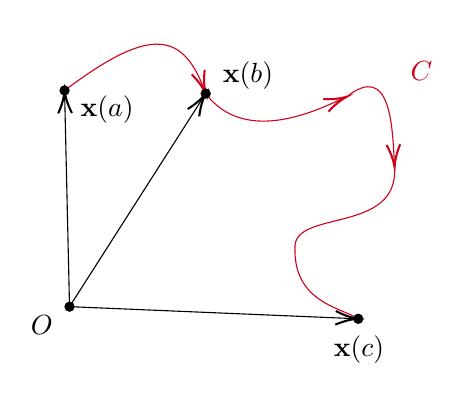
\begin{tikzpicture}[x=0.75pt,y=0.75pt,yscale=-1,xscale=1]
	%uncomment if require: \path (0,300); %set diagram left start at 0, and has height of 300
	
	%Curve Lines [id:da3276060381490892] 
	\draw [color={rgb, 255:red, 208; green, 2; blue, 27 }  ,draw opacity=1 ]   (176,103.75) .. controls (195.37,129.27) and (231.27,111.02) .. (242.33,105.98) ;
	\draw [shift={(244,105.25)}, rotate = 517.62] [color={rgb, 255:red, 208; green, 2; blue, 27 }  ,draw opacity=1 ][line width=0.75]    (10.93,-3.29) .. controls (6.95,-1.4) and (3.31,-0.3) .. (0,0) .. controls (3.31,0.3) and (6.95,1.4) .. (10.93,3.29)   ;
	%Curve Lines [id:da867110150451944] 
	\draw [color={rgb, 255:red, 208; green, 2; blue, 27 }  ,draw opacity=1 ]   (244,105.25) .. controls (264.86,88.76) and (265.95,118.37) .. (266.91,137.51) ;
	\draw [shift={(267,139.25)}, rotate = 266.99] [color={rgb, 255:red, 208; green, 2; blue, 27 }  ,draw opacity=1 ][line width=0.75]    (10.93,-3.29) .. controls (6.95,-1.4) and (3.31,-0.3) .. (0,0) .. controls (3.31,0.3) and (6.95,1.4) .. (10.93,3.29)   ;
	%Curve Lines [id:da48281776098084617] 
	\draw [color={rgb, 255:red, 208; green, 2; blue, 27 }  ,draw opacity=1 ]   (267,139.25) .. controls (269,171.75) and (218,159.25) .. (219,178.25) .. controls (218.5,204.25) and (241,206.75) .. (249.5,212.25) ;
	%Shape: Circle [id:dp01912153166389552] 
	\draw  [draw opacity=0][fill={rgb, 255:red, 0; green, 0; blue, 0 }  ,fill opacity=1 ] (107.9,206.4) .. controls (107.9,205.02) and (109.02,203.9) .. (110.4,203.9) .. controls (111.78,203.9) and (112.9,205.02) .. (112.9,206.4) .. controls (112.9,207.78) and (111.78,208.9) .. (110.4,208.9) .. controls (109.02,208.9) and (107.9,207.78) .. (107.9,206.4) -- cycle ;
	%Curve Lines [id:da9083644795099863] 
	\draw [color={rgb, 255:red, 208; green, 2; blue, 27 }  ,draw opacity=1 ]   (108,102.25) .. controls (147.2,72.85) and (164.31,72.26) .. (175.33,101.9) ;
	\draw [shift={(176,103.75)}, rotate = 250.75] [color={rgb, 255:red, 208; green, 2; blue, 27 }  ,draw opacity=1 ][line width=0.75]    (10.93,-3.29) .. controls (6.95,-1.4) and (3.31,-0.3) .. (0,0) .. controls (3.31,0.3) and (6.95,1.4) .. (10.93,3.29)   ;
	%Shape: Circle [id:dp4960073350824441] 
	\draw  [draw opacity=0][fill={rgb, 255:red, 0; green, 0; blue, 0 }  ,fill opacity=1 ] (105.5,102.25) .. controls (105.5,100.87) and (106.62,99.75) .. (108,99.75) .. controls (109.38,99.75) and (110.5,100.87) .. (110.5,102.25) .. controls (110.5,103.63) and (109.38,104.75) .. (108,104.75) .. controls (106.62,104.75) and (105.5,103.63) .. (105.5,102.25) -- cycle ;
	%Shape: Circle [id:dp8712280703593382] 
	\draw  [draw opacity=0][fill={rgb, 255:red, 0; green, 0; blue, 0 }  ,fill opacity=1 ] (173.5,103.75) .. controls (173.5,102.37) and (174.62,101.25) .. (176,101.25) .. controls (177.38,101.25) and (178.5,102.37) .. (178.5,103.75) .. controls (178.5,105.13) and (177.38,106.25) .. (176,106.25) .. controls (174.62,106.25) and (173.5,105.13) .. (173.5,103.75) -- cycle ;
	%Shape: Circle [id:dp9346879620682326] 
	\draw  [draw opacity=0][fill={rgb, 255:red, 0; green, 0; blue, 0 }  ,fill opacity=1 ] (247,212.25) .. controls (247,210.87) and (248.12,209.75) .. (249.5,209.75) .. controls (250.88,209.75) and (252,210.87) .. (252,212.25) .. controls (252,213.63) and (250.88,214.75) .. (249.5,214.75) .. controls (248.12,214.75) and (247,213.63) .. (247,212.25) -- cycle ;
	%Straight Lines [id:da3352312418861193] 
	\draw    (110.4,206.4) -- (247.5,212.17) ;
	\draw [shift={(249.5,212.25)}, rotate = 182.41] [color={rgb, 255:red, 0; green, 0; blue, 0 }  ][line width=0.75]    (10.93,-3.29) .. controls (6.95,-1.4) and (3.31,-0.3) .. (0,0) .. controls (3.31,0.3) and (6.95,1.4) .. (10.93,3.29)   ;
	%Straight Lines [id:da01233126994686784] 
	\draw    (110.4,206.4) -- (174.92,105.44) ;
	\draw [shift={(176,103.75)}, rotate = 482.58] [color={rgb, 255:red, 0; green, 0; blue, 0 }  ][line width=0.75]    (10.93,-3.29) .. controls (6.95,-1.4) and (3.31,-0.3) .. (0,0) .. controls (3.31,0.3) and (6.95,1.4) .. (10.93,3.29)   ;
	%Straight Lines [id:da11748387967404772] 
	\draw    (110.4,206.4) -- (108.05,104.25) ;
	\draw [shift={(108,102.25)}, rotate = 448.68] [color={rgb, 255:red, 0; green, 0; blue, 0 }  ][line width=0.75]    (10.93,-3.29) .. controls (6.95,-1.4) and (3.31,-0.3) .. (0,0) .. controls (3.31,0.3) and (6.95,1.4) .. (10.93,3.29)   ;
	
	% Text Node
	\draw (90.5,209.5) node [anchor=north west][inner sep=0.75pt]    {$O$};
	% Text Node
	\draw (114.5,103.5) node [anchor=north west][inner sep=0.75pt]    {$\mathbf{x}( a)$};
	% Text Node
	\draw (183,87.25) node [anchor=north west][inner sep=0.75pt]    {$\mathbf{x}( b)$};
	% Text Node
	\draw (236.5,219) node [anchor=north west][inner sep=0.75pt]    {$\mathbf{x}( c)$};
	% Text Node
	\draw (273.5,87) node [anchor=north west][inner sep=0.75pt]  [color={rgb, 255:red, 208; green, 2; blue, 27 }  ,opacity=1 ]  {$C$};
	
	
	\end{tikzpicture}

\end{center}

\begin{definition}[Differentiability and Smoothness]
	We say that a curve $C$ is \vocab{differentiable} if each of the components $\{x_1(t), x_2(t), x_3(t) \}$ are differentiable, and say $C$ is \vocab{regular} if $|\vv{x}'(t)| \neq 0$. If $C$ is differentiable and regular then we say $C$ is \vocab{smooth}.
\end{definition}

\begin{remark}
	The `regular' condition exists to avoid `spikes' in the curve. For example, consider the curve $\vv{x}(t) = (t^3, t^2)$. Clearly this is differentiable, but $\vv{x}(t)$ has a cusp at $t = 0$. At $t = 0$, we have $|\vv{x}(0)| = 0$. If this was not the case, there would be no cusp.
\begin{center}
	\begin{asy}
		unitsize(55);
		import graph;
		pair F(real t) {
			return (t^3, t^2);
		}

		path g = graph(F, -1.1, 1.1);

		draw(g, blue + linewidth(0.9pt));

		draw((0, -0.25) -- (0, 1.2), arrow=Arrow(TeXHead));
		draw((-1.3, 0) -- (1.3, 0), arrow=Arrow(TeXHead));
	\end{asy}
\end{center}

\end{remark}


Recall that the function $x_i(t)$ is differentiable at $t$ if $x_i(t + h) = x_i(t) + x_i'(t) h + o(h)$, where $\frac{o(h)}{h} \rightarrow 0$ as $h \rightarrow 0$. We can write this in terms of vectors, where
$$
\vv{x}(t + h) = \vv{x}(t) + \vv{x}'(t)h + o(h),
$$
where $o(h)$ is a vector for which $\frac{|o(h)|}{h} \rightarrow 0$ as $h \rightarrow 0$.
  
Now given some curve $C$, we may want to find the length of the curve. We can try to do this by approximating the curve using straight lines.

\begin{center}
	

\tikzset{every picture/.style={line width=0.75pt}} %set default line width to 0.75pt        

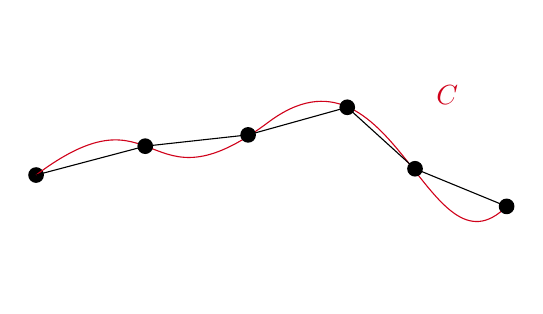
\begin{tikzpicture}[x=0.75pt,y=0.75pt,yscale=-1,xscale=1]
%uncomment if require: \path (0,300); %set diagram left start at 0, and has height of 300

%Shape: Ellipse [id:dp6464695455275871] 
\draw  [draw opacity=0][fill={rgb, 255:red, 0; green, 0; blue, 0 }  ,fill opacity=1 ] (42.5,126.68) .. controls (42.5,124.59) and (44.19,122.9) .. (46.28,122.9) .. controls (48.37,122.9) and (50.06,124.59) .. (50.06,126.68) .. controls (50.06,128.77) and (48.37,130.46) .. (46.28,130.46) .. controls (44.19,130.46) and (42.5,128.77) .. (42.5,126.68) -- cycle ;
%Curve Lines [id:da6916953701818653] 
\draw [color={rgb, 255:red, 208; green, 2; blue, 27 }  ,draw opacity=1 ]   (46.28,126.68) .. controls (106.73,81.34) and (97.66,146.63) .. (158.12,101.29) .. controls (218.57,55.95) and (235.2,179.58) .. (272.98,141.79) ;
%Shape: Circle [id:dp8157615548797015] 
\draw  [draw opacity=0][fill={rgb, 255:red, 0; green, 0; blue, 0 }  ,fill opacity=1 ] (95.09,112.77) .. controls (95.09,110.69) and (96.79,109) .. (98.87,109) .. controls (100.96,109) and (102.65,110.69) .. (102.65,112.77) .. controls (102.65,114.86) and (100.96,116.55) .. (98.87,116.55) .. controls (96.79,116.55) and (95.09,114.86) .. (95.09,112.77) -- cycle ;
%Shape: Ellipse [id:dp6623880161127722] 
\draw  [draw opacity=0][fill={rgb, 255:red, 0; green, 0; blue, 0 }  ,fill opacity=1 ] (144.67,107.33) .. controls (144.67,105.25) and (146.36,103.56) .. (148.45,103.56) .. controls (150.53,103.56) and (152.22,105.25) .. (152.22,107.33) .. controls (152.22,109.42) and (150.53,111.11) .. (148.45,111.11) .. controls (146.36,111.11) and (144.67,109.42) .. (144.67,107.33) -- cycle ;
%Shape: Ellipse [id:dp947023885876757] 
\draw  [draw opacity=0][fill={rgb, 255:red, 0; green, 0; blue, 0 }  ,fill opacity=1 ] (192.43,94.03) .. controls (192.43,91.95) and (194.12,90.26) .. (196.2,90.26) .. controls (198.29,90.26) and (199.98,91.95) .. (199.98,94.03) .. controls (199.98,96.12) and (198.29,97.81) .. (196.2,97.81) .. controls (194.12,97.81) and (192.43,96.12) .. (192.43,94.03) -- cycle ;
%Shape: Ellipse [id:dp9991347478656615] 
\draw  [draw opacity=0][fill={rgb, 255:red, 0; green, 0; blue, 0 }  ,fill opacity=1 ] (225.07,123.66) .. controls (225.07,121.57) and (226.76,119.88) .. (228.85,119.88) .. controls (230.94,119.88) and (232.63,121.57) .. (232.63,123.66) .. controls (232.63,125.74) and (230.94,127.43) .. (228.85,127.43) .. controls (226.76,127.43) and (225.07,125.74) .. (225.07,123.66) -- cycle ;
%Shape: Ellipse [id:dp5868702964474427] 
\draw  [draw opacity=0][fill={rgb, 255:red, 0; green, 0; blue, 0 }  ,fill opacity=1 ] (269.2,141.79) .. controls (269.2,139.71) and (270.89,138.01) .. (272.98,138.01) .. controls (275.07,138.01) and (276.76,139.71) .. (276.76,141.79) .. controls (276.76,143.88) and (275.07,145.57) .. (272.98,145.57) .. controls (270.89,145.57) and (269.2,143.88) .. (269.2,141.79) -- cycle ;
%Straight Lines [id:da7875885498839282] 
\draw    (46.28,126.68) -- (98.87,112.77) ;
%Straight Lines [id:da309124837435779] 
\draw    (98.87,112.77) -- (148.45,107.33) ;
%Straight Lines [id:da8902322155826599] 
\draw    (148.45,107.33) -- (196.2,94.03) ;
%Straight Lines [id:da9085782113625647] 
\draw    (196.2,94.03) -- (228.85,123.66) ;
%Straight Lines [id:da7165214688732946] 
\draw    (228.85,123.66) -- (272.98,141.79) ;

% Text Node
\draw (237.91,82.51) node [anchor=north west][inner sep=0.75pt]  [color={rgb, 255:red, 208; green, 2; blue, 27 }  ,opacity=1 ]  {$C$};


\end{tikzpicture}

\end{center}

For $C:[a, b] \rightarrow \R^3$ with $t \mapsto \vv{x}(t)$, we introduce a partition $P$ of $[a, b]$ with $t_0$, $t_N = b$ and $t_0 < t_1 < \dots < t_N$, and we set $\Delta t_i = t_{i + 1} - t_i$ and $\Delta t = \max_i \Delta t_i$.

\begin{definition}[Length Relative to a Partition]
	For some curve $C$ and partition $P$ as above, we define the \vocab{length} of $C$ relative to $P$ by
	$$
	\ell(C, P) = \sum_{i = 0}^{N - 1} \left|\vv{x}(t_{i + 1}) - \vv{x}(t_i)\right|.
$$
\end{definition}

We would expect that this length would get closer to the true length of $C$ as $\Delta t \rightarrow 0$. Indeed, we will define the length of $C$ in this way.

\begin{definition}[Length of a Curve]
	We define the length of a curve $C$ by
	$$
	\ell(C) = \lim_{\Delta t \to 0} \sum_{i = 0}^{N - 1} \left|\vv{x}(t_{i + 1}) - \vv{x}(t_i) \right| = \lim_{\Delta t \rightarrow 0} \ell(C, P).
	$$
	if this limit does not exist, we say the curve is \vocab{non-rectifiable}.
\end{definition}

In this course, we will not worry too much about non-rectifiable curves, so we will assume that this notion is always well defined.

Now suppose $C$ is a differentiable curve. Then we have that
\begin{align*}
	\vv{x}(t_{i + 1}) &= \vv{x}(t_i + t_{i + 1} - t_i) \\
					&= \vv{x}(t_i + \Delta t_i) \\
					&= \vv{x}(t_i) + \vv{x}'(t_i) \Delta t_i + o(\Delta t_i).
\end{align*}
It follows that
$$
|\vv{x}(t_{i + 1}) - \vv{x}(t_i) | = |\vv{x}'(t_i)| \Delta t_i + o(\Delta t_i). 
$$

So if $C$ is differentiable, we get the expression
$$
\ell(C, P)=\sum_{i=0}^{N-1}\left(\left|\mathbf{x}^{\prime}\left(t_{i}\right)\right| \Delta t_{i}+o\left(\Delta t_{i}\right)\right).
$$
Recall that $o(\Delta t_i)$ represents a function for which $\frac{o(\Delta t_i)}{\Delta t_i} \rightarrow 0$ as $\delta t_i \rightarrow 0$. So for any $\epsilon > 0$, if $\Delta t = \max_i \Delta t_i$  is sufficiently small, then we have
$$
|o(\Delta t_i) | < \left(\frac{\epsilon}{b - a}\right) \Delta t_i,
$$
for $i = \{0, \dots, N - 1\}$. So
\begin{align*}
	\left|\ell(C, P) - \sum_{i = 0}^{N - 1} |\vv{x}' (t_i) \Delta t_i \right| &= \left|\sum_{i = 0}^{N - 1} o(\Delta t_i)\right| \\
	&< \frac{\epsilon}{b - a} \sum_{i = 0}^{N - 1} \Delta{t_i} = \epsilon.
\end{align*}
Thus the LHS tends to zero as $\Delta t \rightarrow 0$. So we get that
\begin{align*}
	\ell(C) &= \lim_{\Delta t \to 0} \ell(C, P) = \lim_{\Delta t \to 0} \sum_{i = 0}^{N - 1} |\vv{x}'(t_i)| \Delta t_i \\
		&= \int_a^b \left|\vv{x}'(t)\right| \; \dd t,
\end{align*}
by the definition of the Riemann integral.
So, we can restate our definition in this other form.

\begin{definition}[Length of a Curve]
	If $C: [a, b] \rightarrow \R^3$ is a differentiable curve with $t \mapsto \vv{x}(t)$, then its \vocab{length} is
	$$
	\ell(C) = \int_a^b |\vv{x}'(t)| \; \dd t = \int_C \dd s,
	$$
where $\dd s$ is the \vocab{arc-length element}, $\dd s = |\vv{x}'(t)| \; \dd t$.
\end{definition}

With this defined, we can define the integral of a function along a curve.

\begin{definition}[Integral on a Curve]
	For a function $f : \R^3 \rightarrow \R$ and a differentiable curve $C: [a, b] \rightarrow \R^3$ with $t \mapsto \vv{x}(t)$, we define the \vocab{integral of $f$ along $C$} to be
	$$
	\int_C f(\vv{x})\; \dd s = \int_a^b f(\vv{x}(t)) |\vv{x}'(t)| \; \dd t.
	$$
\end{definition}

Now consider a curve $C$ made up of $M$ smooth curves $C_1, C_2, \dots, C_M$.

\begin{center}
	

\tikzset{every picture/.style={line width=0.75pt}} %set default line width to 0.75pt        

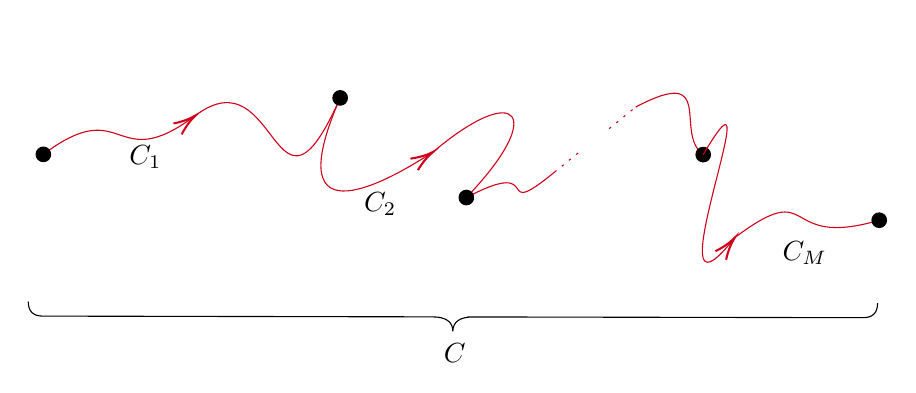
\begin{tikzpicture}[x=0.75pt,y=0.75pt,yscale=-1,xscale=1]
%uncomment if require: \path (0,300); %set diagram left start at 0, and has height of 300

%Curve Lines [id:da5796763237473451] 
\draw [color={rgb, 255:red, 208; green, 2; blue, 27 }  ,draw opacity=1 ]   (37.48,39.48) .. controls (77.08,9.78) and (71.01,49.86) .. (109.69,21.56) ;
\draw [shift={(110.88,20.68)}, rotate = 503.13] [color={rgb, 255:red, 208; green, 2; blue, 27 }  ,draw opacity=1 ][line width=0.75]    (10.93,-3.29) .. controls (6.95,-1.4) and (3.31,-0.3) .. (0,0) .. controls (3.31,0.3) and (6.95,1.4) .. (10.93,3.29)   ;
%Curve Lines [id:da30640590954836433] 
\draw [color={rgb, 255:red, 208; green, 2; blue, 27 }  ,draw opacity=1 ]   (110.88,20.68) .. controls (150.88,-9.32) and (148.48,84.28) .. (180.48,12.28) ;
%Curve Lines [id:da18452242492784054] 
\draw [color={rgb, 255:red, 208; green, 2; blue, 27 }  ,draw opacity=1 ]   (180.48,12.28) .. controls (148.83,84.85) and (206.94,50.14) .. (223.63,39.35) ;
\draw [shift={(225.28,38.28)}, rotate = 506.69] [color={rgb, 255:red, 208; green, 2; blue, 27 }  ,draw opacity=1 ][line width=0.75]    (10.93,-3.29) .. controls (6.95,-1.4) and (3.31,-0.3) .. (0,0) .. controls (3.31,0.3) and (6.95,1.4) .. (10.93,3.29)   ;
%Curve Lines [id:da1500064698451402] 
\draw [color={rgb, 255:red, 208; green, 2; blue, 27 }  ,draw opacity=1 ]   (225.28,38.28) .. controls (266.08,3.88) and (280.08,19.88) .. (241.28,60.28) ;
%Shape: Ellipse [id:dp3321298680409044] 
\draw  [draw opacity=0][fill={rgb, 255:red, 0; green, 0; blue, 0 }  ,fill opacity=1 ] (176.7,12.28) .. controls (176.7,10.19) and (178.39,8.5) .. (180.48,8.5) .. controls (182.57,8.5) and (184.26,10.19) .. (184.26,12.28) .. controls (184.26,14.37) and (182.57,16.06) .. (180.48,16.06) .. controls (178.39,16.06) and (176.7,14.37) .. (176.7,12.28) -- cycle ;
%Shape: Ellipse [id:dp5859967156381527] 
\draw  [draw opacity=0][fill={rgb, 255:red, 0; green, 0; blue, 0 }  ,fill opacity=1 ] (33.7,39.48) .. controls (33.7,37.39) and (35.39,35.7) .. (37.48,35.7) .. controls (39.57,35.7) and (41.26,37.39) .. (41.26,39.48) .. controls (41.26,41.57) and (39.57,43.26) .. (37.48,43.26) .. controls (35.39,43.26) and (33.7,41.57) .. (33.7,39.48) -- cycle ;
%Curve Lines [id:da9173421636172133] 
\draw [color={rgb, 255:red, 208; green, 2; blue, 27 }  ,draw opacity=1 ]   (241.28,60.28) .. controls (280.6,39.6) and (253,73.2) .. (283.8,48) ;
%Shape: Ellipse [id:dp4659247920376307] 
\draw  [draw opacity=0][fill={rgb, 255:red, 0; green, 0; blue, 0 }  ,fill opacity=1 ] (237.5,60.28) .. controls (237.5,58.19) and (239.19,56.5) .. (241.28,56.5) .. controls (243.37,56.5) and (245.06,58.19) .. (245.06,60.28) .. controls (245.06,62.37) and (243.37,64.06) .. (241.28,64.06) .. controls (239.19,64.06) and (237.5,62.37) .. (237.5,60.28) -- cycle ;
%Straight Lines [id:da8487824909604982] 
\draw [color={rgb, 255:red, 208; green, 2; blue, 27 }  ,draw opacity=1 ] [dash pattern={on 0.84pt off 2.51pt}]  (283.8,48) -- (296.6,37.6) ;
%Curve Lines [id:da5732848696347904] 
\draw [color={rgb, 255:red, 208; green, 2; blue, 27 }  ,draw opacity=1 ]   (322.88,16.68) .. controls (362.2,-4) and (341,29.2) .. (355.4,39.6) ;
%Straight Lines [id:da9728872621803147] 
\draw [color={rgb, 255:red, 208; green, 2; blue, 27 }  ,draw opacity=1 ] [dash pattern={on 0.84pt off 2.51pt}]  (310.08,27.08) -- (322.88,16.68) ;
%Shape: Ellipse [id:dp6071568671300255] 
\draw  [draw opacity=0][fill={rgb, 255:red, 0; green, 0; blue, 0 }  ,fill opacity=1 ] (351.62,39.6) .. controls (351.62,37.51) and (353.31,35.82) .. (355.4,35.82) .. controls (357.49,35.82) and (359.18,37.51) .. (359.18,39.6) .. controls (359.18,41.69) and (357.49,43.38) .. (355.4,43.38) .. controls (353.31,43.38) and (351.62,41.69) .. (351.62,39.6) -- cycle ;
%Curve Lines [id:da29258101011575044] 
\draw [color={rgb, 255:red, 208; green, 2; blue, 27 }  ,draw opacity=1 ]   (355.4,39.6) .. controls (391.22,-21.29) and (328.04,132.85) .. (369.96,80.41) ;
\draw [shift={(370.6,79.6)}, rotate = 488.25] [color={rgb, 255:red, 208; green, 2; blue, 27 }  ,draw opacity=1 ][line width=0.75]    (10.93,-3.29) .. controls (6.95,-1.4) and (3.31,-0.3) .. (0,0) .. controls (3.31,0.3) and (6.95,1.4) .. (10.93,3.29)   ;
%Curve Lines [id:da6819173648579594] 
\draw [color={rgb, 255:red, 208; green, 2; blue, 27 }  ,draw opacity=1 ]   (370.6,79.6) .. controls (410.6,49.6) and (391.4,85.6) .. (440.2,71.2) ;
%Shape: Ellipse [id:dp5818550932291585] 
\draw  [draw opacity=0][fill={rgb, 255:red, 0; green, 0; blue, 0 }  ,fill opacity=1 ] (436.42,71.2) .. controls (436.42,69.11) and (438.11,67.42) .. (440.2,67.42) .. controls (442.29,67.42) and (443.98,69.11) .. (443.98,71.2) .. controls (443.98,73.29) and (442.29,74.98) .. (440.2,74.98) .. controls (438.11,74.98) and (436.42,73.29) .. (436.42,71.2) -- cycle ;
%Shape: Brace [id:dp414059666657298] 
\draw   (30.2,110.4) .. controls (30.19,115.07) and (32.52,117.4) .. (37.19,117.41) -- (224.79,117.77) .. controls (231.46,117.78) and (234.78,120.12) .. (234.77,124.79) .. controls (234.78,120.12) and (238.12,117.8) .. (244.79,117.81)(241.79,117.81) -- (432.39,118.17) .. controls (437.06,118.18) and (439.39,115.86) .. (439.4,111.19) ;

% Text Node
\draw (77.6,34) node [anchor=north west][inner sep=0.75pt]    {$C_{1}$};
% Text Node
\draw (190.8,56.4) node [anchor=north west][inner sep=0.75pt]    {$C_{2}$};
% Text Node
\draw (229.2,129.6) node [anchor=north west][inner sep=0.75pt]    {$C$};
% Text Node
\draw (392.4,80.4) node [anchor=north west][inner sep=0.75pt]    {$C_{M}$};


\end{tikzpicture}

\end{center}

Then writing $C = C_1 + C_2 + \cdots + C_M$, we can define
$$
\int_C f(\vv{x}) \; \dd s = \sum_{i = 1}^M \int_{C_i} f(\vv{x}) \; \dd s,
$$
so we can integrate over piecewise smooth curves.

Note that informally, we have 
$$\dd s = |\vv{x}'(t)| \; \dd t = \sqrt{\left(\frac{\dd x}{\dd t}\right)^2 + \left(\frac{\dd y}{\dd t}\right)^2 + \left(\frac{\dd z}{\dd t}\right)^2} \; \dd t.$$
So being somewhat sacrilegious, we have
$$
\dd s^2 = \dd x^2 + \dd y^2 + \dd z^2.
$$

\begin{example}[Circumference of a Circle]
	Let $C$ be a circle of radius $r > 0$ in $\R^3$,
	$$
	\vv{x}(t) = \begin{pmatrix}
		r \cos t \\
		r \sin t \\
		0
	\end{pmatrix}, \quad \quad t \in [0, 2 \pi].
	$$
	We can differentiate this to get 
	$$
	\vv{x}'(t) = \begin{pmatrix}
		-r \sin t \\
		r \cos t \\
		0
	\end{pmatrix}, \quad \quad t \in [0, 2 \pi].
	$$
	Then integrating over $C$ we have
	\begin{align*}
		\int_C \; \dd s &= \int_0^{2 \pi} \sqrt{r^2 \sin^2 t + r^2 \cos^2 t} \; \dd t\\
		&= \int_0^{2 \pi} r \; \dd t \\
		&= 2 \pi r,
	\end{align*}
	as we would expect.
\end{example}

\begin{example}[Integrating over a Circle]
	With $C$ being a circle as before, we can integrate over the curve. For example
	\begin{align*}
		\int_C x^2 y \; \dd s &= \int_0^{2 \pi} (r \cos t)^2 (r \sin t) \underbrace{r \; \dd t}_{|\vv{x}'(t)| \; \dd t} \\
		&= 0
	\end{align*}
\end{example}

There is one subtlety that we have looked over - does $\ell(C)$ depend on the parameterization used?

For example, if we had $\vv{x}(t) = (r \cos t, r \sin t, 0)$ with $t \in [0, 2 \pi]$ and $\tilde{\vv{x}}(t) = (r \cos(2 t), r \sin(2 t), 0)$ with $t \in [0, \pi]$, these represent the same circle and they should have the same length. We will clear up this possible ambiguity now.

\begin{proposition}
	If $f:\R^3 \rightarrow \R$ is a function and $C$ is a differentiable curve, then $\int_C f(\vv{x}) \; \dd s$ is independent of the parameterization of $C$ used.
\end{proposition}
\begin{proof}
Suppose $C$ has two different parameterization,
\begin{align*}
	\vv{x} &= \vv{x}_1(t), \quad \quad a \leq t \leq b \\
	\vv{x} &= \vv{x}_2(t), \quad \quad \alpha \leq t \leq \beta
\end{align*}
We must then have $\vv{x}_2(\tau) = \vv{x}_1(t(\tau))$ for some function $t(\tau)$. We can assume that $\frac{\dd t}{\dd \tau} \neq 0$ so the map between $t$ and $\tau$ is invertible and differentiable (this is the inverse function theorem, covered in Analysis and Topology in Part IB). Note then that 
\begin{align*}
	\vv{x}'_2(\tau) &= \frac{\dd}{\dd\tau} \vv{x}_2(t) \\
	&= \frac{\dd} {\dd \tau} \vv{x}_1(t(\tau)) \\
	&= \frac{\dd t}{\dd \tau} \vv{x}_1'(t(\tau)).
\end{align*}
Then from our definition,
$$
\int_C f(\vv{x}) \; \dd s = \int_{a}^b f(\vv{x}_1(t)) |\vv{x}_1'(t)| \; \dd t.
$$
We can make the substitution $t = t(\tau)$, and assuming $\dd t/\dd\tau > 0$, the later integral becomes
$$
\int_\alpha^\beta f(\vv{x}_2(\tau)) \underbrace{|\vv{x}_1'(t(\tau))| \frac{\dd t}{\dd \tau} \;\dd \tau}_{|\vv{x}'_2 (\tau)| \; \dd\tau},
$$
which is precisely the same as $\int_C f(\vv{x}) \; \dd s$ using the $\vv{x}_2(t)$ parameterization. 

We assumed here that $\frac{\dd t}{\dd \tau} > 0$, but the same holds if it is negative. Thus our definition of integrating over a curve $C$ does not depend on the choice of parameterization of $C$.
\end{proof}

We can parameterize curves in many different ways. One useful way to parameterise regular cuves is with respect to arc-length.
If we write $\vv{r}(s) = \vv{x}(t(s))$ where $0 \leq s \leq \ell(C)$, then by the chain rule
$$
	\frac{\dd t}{\dd s} = \frac{1}{\dd s/ \dd t} = \frac{1}{|\vv{x}'(t(s))|},
$$
so
\begin{align*}
	\vv{r}'(s) &= \frac{\dd}{\dd s} \vv{x}(t(s)) \\
	&= \frac{\dd t}{\d d s} \vv{x}'(t(s)) \\
	&= \frac{\vv{x}'(t(s_))}{|\vv{x}'(t(s))|},
\end{align*}
that is, $|\vv{r}'(s)| = 1$. This (consistently) gives $\ell(C) = \int_0^{\ell(C)} |\vv{r}'(s)| \; \dd s) = \int_0^{\ell(C)} \; \dd s$.
So the way to picture $\vv{r}'(s)$ is as the unit tangent vector to the curve.

\begin{center}
	

\tikzset{every picture/.style={line width=0.75pt}} %set default line width to 0.75pt        

\begin{tikzpicture}[x=0.75pt,y=0.75pt,yscale=-1,xscale=1]
%uncomment if require: \path (0,300); %set diagram left start at 0, and has height of 300

%Shape: Ellipse [id:dp6228782401096558] 
\draw  [draw opacity=0][fill={rgb, 255:red, 0; green, 0; blue, 0 }  ,fill opacity=1 ] (158.04,210.31) .. controls (158.04,208.37) and (159.61,206.8) .. (161.54,206.8) .. controls (163.48,206.8) and (165.05,208.37) .. (165.05,210.31) .. controls (165.05,212.24) and (163.48,213.81) .. (161.54,213.81) .. controls (159.61,213.81) and (158.04,212.24) .. (158.04,210.31) -- cycle ;
%Straight Lines [id:da8695480911058163] 
\draw    (161.54,210.31) -- (156.84,56.82) ;
\draw [shift={(156.78,54.82)}, rotate = 448.24] [color={rgb, 255:red, 0; green, 0; blue, 0 }  ][line width=0.75]    (10.93,-3.29) .. controls (6.95,-1.4) and (3.31,-0.3) .. (0,0) .. controls (3.31,0.3) and (6.95,1.4) .. (10.93,3.29)   ;
%Curve Lines [id:da8139461687050455] 
\draw [color={rgb, 255:red, 208; green, 2; blue, 27 }  ,draw opacity=1 ]   (67.05,164.18) .. controls (64.24,127.73) and (111.91,53.42) .. (158.18,54.82) .. controls (204.45,56.22) and (203.05,168.39) .. (291.38,95.48) ;
%Straight Lines [id:da9732872849600818] 
\draw    (161.54,210.31) -- (68.84,165.06) ;
\draw [shift={(67.05,164.18)}, rotate = 386.02] [color={rgb, 255:red, 0; green, 0; blue, 0 }  ][line width=0.75]    (10.93,-3.29) .. controls (6.95,-1.4) and (3.31,-0.3) .. (0,0) .. controls (3.31,0.3) and (6.95,1.4) .. (10.93,3.29)   ;
%Straight Lines [id:da38328258500214996] 
\draw [color={rgb, 255:red, 74; green, 144; blue, 226 }  ,draw opacity=1 ]   (67.05,164.18) -- (63.55,117.52) ;
\draw [shift={(63.4,115.53)}, rotate = 445.71] [color={rgb, 255:red, 74; green, 144; blue, 226 }  ,draw opacity=1 ][line width=0.75]    (10.93,-3.29) .. controls (6.95,-1.4) and (3.31,-0.3) .. (0,0) .. controls (3.31,0.3) and (6.95,1.4) .. (10.93,3.29)   ;
%Straight Lines [id:da8330115590680308] 
\draw [color={rgb, 255:red, 74; green, 144; blue, 226 }  ,draw opacity=1 ]   (156.78,54.82) -- (204.97,57.65) ;
\draw [shift={(206.97,57.76)}, rotate = 183.36] [color={rgb, 255:red, 74; green, 144; blue, 226 }  ,draw opacity=1 ][line width=0.75]    (10.93,-3.29) .. controls (6.95,-1.4) and (3.31,-0.3) .. (0,0) .. controls (3.31,0.3) and (6.95,1.4) .. (10.93,3.29)   ;

% Text Node
\draw (163.54,213.31) node [anchor=north west][inner sep=0.75pt]    {$O$};
% Text Node
\draw (293.38,98.48) node [anchor=north west][inner sep=0.75pt]  [color={rgb, 255:red, 208; green, 2; blue, 27 }  ,opacity=1 ]  {$C$};
% Text Node
\draw (94.62,190.95) node [anchor=north west][inner sep=0.75pt]  [color={rgb, 255:red, 0; green, 0; blue, 0 }  ,opacity=1 ]  {$\mathbf{r}( 0)$};
% Text Node
\draw (32.22,92.95) node [anchor=north west][inner sep=0.75pt]  [color={rgb, 255:red, 74; green, 144; blue, 226 }  ,opacity=1 ]  {$\mathbf{r} '( 0)$};
% Text Node
\draw (160.62,30.55) node [anchor=north west][inner sep=0.75pt]  [color={rgb, 255:red, 74; green, 144; blue, 226 }  ,opacity=1 ]  {$\mathbf{r} '( s)$};
% Text Node
\draw (161.82,115.75) node [anchor=north west][inner sep=0.75pt]  [color={rgb, 255:red, 74; green, 144; blue, 226 }  ,opacity=1 ]  {$\mathbf{r}( s)$};


\end{tikzpicture}

\end{center}

\section{Curvature and Torsion}

Throughout this section, 
we  will talk about a generic regular curve $C$, parameterized by arc-length, and we will write $s \mapsto \vv{r}(s).$

\begin{definition}[Tangent Vector]
	For a regular curve $C$ parameterized by arc length, we define the \vocab{tangent vector} to be $\vv{t}(s) = \vv{r}'(s)$.
\end{definition}

We already established that $|\vv{t}(s)| = 1$, and thus as the second derivative $\vv{r}''(s) = \vv{t}'(s)$ only measures the change in \emph{direction}.

Intuitively, if $|\vv{r}''(s)|$ is large, then the curve rapidly changes in direction, whereas if $|\vv{r}''(s)|$ is small, we would expect the curve to be approximately flat.

\begin{definition}[Curvature]
	We define the \vocab{curvature} of $C$ to be $\kappa(s) = |\vv{r}''(s)| = |\vv{t}'(s)|$.
\end{definition}
\begin{center}
	

\tikzset{every picture/.style={line width=0.75pt}} %set default line width to 0.75pt        

\begin{tikzpicture}[x=0.75pt,y=0.75pt,yscale=-1,xscale=1]
%uncomment if require: \path (0,300); %set diagram left start at 0, and has height of 300

%Curve Lines [id:da6272470901360102] 
\draw [color={rgb, 255:red, 208; green, 2; blue, 27 }  ,draw opacity=1 ]   (47,107.6) .. controls (69,113.1) and (130.6,82.2) .. (140,86.5) .. controls (149.4,90.8) and (9.2,128.2) .. (40.2,131.2) ;
%Shape: Circle [id:dp23011696399122117] 
\draw  [color={rgb, 255:red, 0; green, 0; blue, 0 }  ,draw opacity=1 ][dash pattern={on 4.5pt off 4.5pt}] (127.5,86.5) .. controls (127.5,79.6) and (133.1,74) .. (140,74) .. controls (146.9,74) and (152.5,79.6) .. (152.5,86.5) .. controls (152.5,93.4) and (146.9,99) .. (140,99) .. controls (133.1,99) and (127.5,93.4) .. (127.5,86.5) -- cycle ;
%Curve Lines [id:da8187188453621865] 
\draw [color={rgb, 255:red, 208; green, 2; blue, 27 }  ,draw opacity=1 ]   (299.8,102) .. controls (339.4,88) and (415.8,132.4) .. (455.8,102.4) ;
%Shape: Circle [id:dp5617098266931536] 
\draw  [color={rgb, 255:red, 0; green, 0; blue, 0 }  ,draw opacity=1 ][dash pattern={on 4.5pt off 4.5pt}] (363.1,105.7) .. controls (363.1,98.8) and (368.7,93.2) .. (375.6,93.2) .. controls (382.5,93.2) and (388.1,98.8) .. (388.1,105.7) .. controls (388.1,112.6) and (382.5,118.2) .. (375.6,118.2) .. controls (368.7,118.2) and (363.1,112.6) .. (363.1,105.7) -- cycle ;

% Text Node
\draw (148.6,52.4) node [anchor=north west][inner sep=0.75pt]   [align=left] {$\displaystyle \kappa ( s)$ large};
% Text Node
\draw (379,65.2) node [anchor=north west][inner sep=0.75pt]   [align=left] {$\displaystyle \kappa ( s)$ small};


\end{tikzpicture}

\end{center}

Now since $\vv{t} = \vv{r}'(s)$ is a unit vector, if we differentiate $\vv{t} \cdot \vv{t} = 1$ we get $\vv{t} \cdot \vv{t}' = 0$. Because of this we can introduce the following definition.

\begin{definition}[Principle Normal]
	The \vocab{principle normal} $\vv{n}$ is the vector given by $\vv{t}' = \kappa \vv{n}$.
\end{definition}

The principle normal $\vv{n}$ is everywhere normal to the curve $C$, since it's always perpendicular to the tangent vector ($\vv{t} \cdot \vv{n} = 0$). Then we have two perpendicular vectors, so we can extend $\{\vv{t}, \vv{n}\}$ to an orthonormal basis by defining the following.

\begin{definition}[Binormal]
	The \vocab{binormal} $\vv{b}$ is the unit vector perpendicular to $\vv{t}$ and $\vv{n}$, $\vv{b} = \vv{t} \times \vv{n}$. 
\end{definition}

Since $|\vv{b}| = 1$, we have $\vv{b}' \cdot \vv{b} = 0$. Also since $\vv{t} \cdot \vv{b} = 0$ and $\vv{n} \cdot \vv{b} = 0$,
\begin{align*}
	0 &= (\vv{t} \cdot \vv{b})' = \vv{t}' \cdot \vv{b} + \vv{t} \cdot \vv{b}'  \\
	&= \cancel{\kappa \vv{n} \cdot \vv{b}} + \vv{t} \cdot \vv{b}',
\end{align*}
thus $\vv{b}'$ is orthogonal to $\vv{t}$ and $\vv{b}$, and thus it is parallel to $\vv{n}$. We define the following.

\begin{definition}[Torsion]
	We define the \vocab{torsion} $\tau$ by $\vv{b}' = - \tau \vv{n}$.
\end{definition}

Informally, torsion measures a twisting motion along a curve.
So we have two equations.
$$
\vv{t}' = \kappa \vv{n}, \quad \quad \vv{b}' = - \tau \vv{n}.
$$

\begin{proposition}[Fundamental Theorem of Curves]
	The curvature $\kappa(s)$ and torsion $\tau(s)$ define a curve up to translation and orientation.
\end{proposition}
\begin{proof}[Proof Sketch]
	Since $\vv{n} = \vv{b} \times \vv{t}$, we have
	$$
	\vv{t}' = \kappa (\vv{b} \times \vv{t}), \quad \vv{b}' = - \tau (\vv{b} \times \vv{t}).
	$$
	This gives six equations for six unknowns. Given $\kappa(s)$, $\tau(s)$, $\vv{t}(0)$ and $\vv{b}(0)$, we can construct the functions $\vv{t}(s)$, $\vv{b}(s)$, and hence $\vv{n} = \vv{b} \times \vv{t}$. Hence the result.
\end{proof}

\section{Radius of Curvature}

Consider some generic curve $s \mapsto \vv{r}(s)$, and consider the Taylor expansion about $s = 0$. Write $\vv{t} = \vv{t}(0)$, $\vv{n} = \vv{n}(0)$, etc. Then we get
\begin{align*}
	\vv{r}(s) &= \vv{r}(0) + s\vv{r}'(0) + \frac{1}{2}s^2 \vv{r}''(0) + o(s^2) \\
	&= \vv{r} + s\vv{t} + \frac{1}{2}s^2 \kappa \vv{n}	+ o(S^2).
\end{align*}
So this gives us a good approximation of the curve around $s = 0$, and now we want to try and draw a circle through the point $\vv{r}(0)$ such that the circle is tangent to the curve at that point. Specifically, what would the radius of that circle be?

Suppose, without loss of generality, that $\vv{t}$ is horizontal.

\begin{center}
	


	\tikzset{every picture/.style={line width=0.75pt}} %set default line width to 0.75pt        

	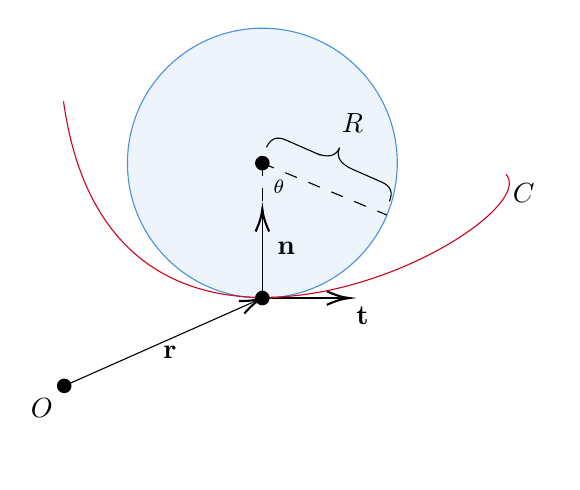
\begin{tikzpicture}[x=0.75pt,y=0.75pt,yscale=-1,xscale=1]
	%uncomment if require: \path (0,300); %set diagram left start at 0, and has height of 300
	
	%Shape: Ellipse [id:dp11623285715454001] 
	\draw  [draw opacity=0][fill={rgb, 255:red, 0; green, 0; blue, 0 }  ,fill opacity=1 ] (161.04,202.31) .. controls (161.04,200.37) and (162.61,198.8) .. (164.54,198.8) .. controls (166.48,198.8) and (168.05,200.37) .. (168.05,202.31) .. controls (168.05,204.24) and (166.48,205.81) .. (164.54,205.81) .. controls (162.61,205.81) and (161.04,204.24) .. (161.04,202.31) -- cycle ;
	%Straight Lines [id:da2508934300022321] 
	\draw    (164.54,202.31) -- (258.17,160.81) ;
	\draw [shift={(260,160)}, rotate = 516.1] [color={rgb, 255:red, 0; green, 0; blue, 0 }  ][line width=0.75]    (10.93,-3.29) .. controls (6.95,-1.4) and (3.31,-0.3) .. (0,0) .. controls (3.31,0.3) and (6.95,1.4) .. (10.93,3.29)   ;
	%Straight Lines [id:da7674997790762081] 
	\draw [color={rgb, 255:red, 0; green, 0; blue, 0 }  ,draw opacity=1 ]   (260,160) -- (300,160) ;
	\draw [shift={(302,160)}, rotate = 180] [color={rgb, 255:red, 0; green, 0; blue, 0 }  ,draw opacity=1 ][line width=0.75]    (10.93,-3.29) .. controls (6.95,-1.4) and (3.31,-0.3) .. (0,0) .. controls (3.31,0.3) and (6.95,1.4) .. (10.93,3.29)   ;
	%Shape: Circle [id:dp6348939130079169] 
	\draw  [color={rgb, 255:red, 74; green, 144; blue, 226 }  ,draw opacity=1 ][fill={rgb, 255:red, 74; green, 144; blue, 226 }  ,fill opacity=0.1 ] (195,95) .. controls (195,59.1) and (224.1,30) .. (260,30) .. controls (295.9,30) and (325,59.1) .. (325,95) .. controls (325,130.9) and (295.9,160) .. (260,160) .. controls (224.1,160) and (195,130.9) .. (195,95) -- cycle ;
	%Straight Lines [id:da4205464127260875] 
	\draw [draw opacity=0]   (260,95) -- (260,160) ;
	\draw [shift={(260,160)}, rotate = 90] [draw opacity=0][line width=0.75]      (0, 0) circle [x radius= 3.35, y radius= 3.35]   ;
	\draw [shift={(260,95)}, rotate = 90] [draw opacity=0][line width=0.75]      (0, 0) circle [x radius= 3.35, y radius= 3.35]   ;
	%Straight Lines [id:da5779811168879634] 
	\draw  [dash pattern={on 4.5pt off 4.5pt}]  (260,95) -- (320,120) ;
	%Straight Lines [id:da25785735111397157] 
	\draw [color={rgb, 255:red, 0; green, 0; blue, 0 }  ,draw opacity=1 ]   (260,160) -- (260,119) ;
	\draw [shift={(260,117)}, rotate = 450] [color={rgb, 255:red, 0; green, 0; blue, 0 }  ,draw opacity=1 ][line width=0.75]    (10.93,-3.29) .. controls (6.95,-1.4) and (3.31,-0.3) .. (0,0) .. controls (3.31,0.3) and (6.95,1.4) .. (10.93,3.29)   ;
	%Shape: Ellipse [id:dp504146351430413] 
	\draw  [draw opacity=0][fill={rgb, 255:red, 0; green, 0; blue, 0 }  ,fill opacity=1 ] (256.49,95) .. controls (256.49,93.06) and (258.06,91.49) .. (260,91.49) .. controls (261.94,91.49) and (263.51,93.06) .. (263.51,95) .. controls (263.51,96.94) and (261.94,98.51) .. (260,98.51) .. controls (258.06,98.51) and (256.49,96.94) .. (256.49,95) -- cycle ;
	%Curve Lines [id:da3234174981600959] 
	\draw [color={rgb, 255:red, 208; green, 2; blue, 27 }  ,draw opacity=1 ]   (164.2,65.2) .. controls (188.2,238.8) and (399.4,124.8) .. (377.4,100.4) ;
	%Shape: Ellipse [id:dp9921539771179669] 
	\draw  [draw opacity=0][fill={rgb, 255:red, 0; green, 0; blue, 0 }  ,fill opacity=1 ] (256.49,160) .. controls (256.49,158.06) and (258.06,156.49) .. (260,156.49) .. controls (261.94,156.49) and (263.51,158.06) .. (263.51,160) .. controls (263.51,161.94) and (261.94,163.51) .. (260,163.51) .. controls (258.06,163.51) and (256.49,161.94) .. (256.49,160) -- cycle ;
	%Shape: Brace [id:dp6625426388074377] 
	\draw   (321.2,113.4) .. controls (323.07,109.13) and (321.88,106.05) .. (317.61,104.18) -- (303.57,98.01) .. controls (297.46,95.33) and (295.35,91.85) .. (297.23,87.58) .. controls (295.35,91.85) and (291.36,92.65) .. (285.26,89.97)(288.01,91.18) -- (271.22,83.81) .. controls (266.95,81.93) and (263.87,83.13) .. (262,87.4) ;
	%Straight Lines [id:da3029069687640311] 
	\draw  [dash pattern={on 4.5pt off 4.5pt}]  (260,95) -- (260,117) ;
	
	% Text Node
	\draw (379.4,103.4) node [anchor=north west][inner sep=0.75pt]    {$C$};
	% Text Node
	\draw (147.2,207.2) node [anchor=north west][inner sep=0.75pt]    {$O$};
	% Text Node
	\draw (211,182) node [anchor=north west][inner sep=0.75pt]    {$\mathbf{r}$};
	% Text Node
	\draw (304,163) node [anchor=north west][inner sep=0.75pt]  [color={rgb, 255:red, 0; green, 0; blue, 0 }  ,opacity=1 ]  {$\mathbf{t}$};
	% Text Node
	\draw (264,102) node [anchor=north west][inner sep=0.75pt]  [font=\scriptsize]  {$\theta $};
	% Text Node
	\draw (266,132) node [anchor=north west][inner sep=0.75pt]  [color={rgb, 255:red, 0; green, 0; blue, 0 }  ,opacity=1 ]  {$\mathbf{n}$};
	% Text Node
	\draw (297,70) node [anchor=north west][inner sep=0.75pt]    {$R$};
	
	
	\end{tikzpicture}
	

\end{center}
A point on this circle can be described by
$$
\vv{x}(\theta) = \vv{r} + R(1 - \cos \theta) \vv{n} + R \sin \theta \vv{t}.
$$
Then expanding for $|\theta|$ small, we get
$$
\vv{x} (\theta) = \vv{r} + R \theta \vv{t} + \frac{1}{2} R \theta^2 \vv{n} + o(\theta^2).
$$
On this circle, the arc-length is $s = R \theta$. Thus if we express the above in terms of arc-length, we get
$$
\vv{x}(\theta) = \vv{r} + S \vv{t} + \frac{1}{2R} s^2 \vv{n} + o(s^2).
$$
As we want this to match the curve, we compare it to the equation for the curve near $\vv{r}$, and to match quadratic terms we need
$R = 1/\kappa$.

\begin{definition}[Radius of Curvature]
	We define $R(s)=1/\kappa(s)$ to be the \vocab{radius of curvature} of the curve $s \mapsto \vv{r}(s)$.
\end{definition}

\chapter{Coordinates, Differentials and Gradients}

\section{Differentials and First Order Changes}

Recall that for $f = f(u_1, \dots, u_n)$, we define the \vocab{differential} of $f$, written $\dd f$, by
$$
\dd f = \frac{\partial f}{\partial u_i} \dd u_i,
$$
using the summation convention. We call $\{\dd u_i\}$ \vocab{differential forms}. We will treat these differential forms as formal objects that are the elements of some abstract vector space, and treat them as linear independent if $\{u_1,  \dots, u_n\}$ are independent, that is, if $\alpha_i \dd u_i = 0$ implies $\alpha_i = 0$ for $i = 1, \dots, n$.

Similarity, if we had $\vv{x} = \vv{x}(u_1, \dots, u_n)$, we define
$$
\dd \vv{x} = \frac{\partial \vv{x}}{\partial u_i} \dd u_i.
$$

\begin{example}[Using Differentials]
	If $f(u, v, w) = u^2 + w\sin(v)$, then
	$$
	\dd f = 2 u \dd u + w \cos (v) \dd v + \sin (v) \dd w.
$$
Similarity, if we had $\vv{x}(u, v, w) = \begin{pmatrix}
	u^2 - v^2 \\ w \\ e^v
\end{pmatrix}$, then
$$
\dd \vv{x} = \begin{pmatrix}
	2u \\ 0 \\ 0\end{pmatrix}
 \dd u + \begin{pmatrix}
	 - 2v \\ 0 \\ e^v
 \end{pmatrix} \dd v + \begin{pmatrix}
	 0 \\ 1 \\ 0
 \end{pmatrix} \dd w.
$$
\end{example}

Differentials encode information about how a function/field changes when we `wobble' our coordinates. Indeed, by calculus we know
$$
f(u_1 + \delta u_1, \dots, u_n + \delta u_n) - f(u_1, \dots, u_n) = \frac{\partial f}{\partial u_i} \delta u_i + o(\delta \vv{u}),
$$
where $\delta\vv{u} = (\delta u_1, \dots, \delta u_n)$. So differentials allow to discuss first order changes in $f$.

So if $\delta f$ denotes a change in $f(u_1, \dots, u_n)$ under perturbation of coordinates $(u_1, \dots, u_n) \mapsto (u_1 + \delta u_1, \dots, u_n + \delta u_n)$,  we have, to first order,
$$
\delta f \approx \frac{\partial f}{\partial u_i} \delta u_i.
$$

Similarly for vector fields,
$$
\delta \vv{x} \approx \frac{\partial \vv{x}}{\partial u_i} \delta u_i.
$$

\section{Coordinates and Line Elements}

You have already seen at least two sets of coordinates before taking this course for $\R^2$: Cartesian coordinates $(x, y)$, and polar coordinates $(r, \theta)$. They have an invertible (except at the origin) relationship,
$$
x = r \cos \theta, y = r \sin \theta.
$$


A general set of coordinates $(u, v)$ on $\R^2$ can be specified by their relationship to $(x, y)$, the Cartesian coordinates. That is, we can specify smooth functions $x = x(u, v)$, $y = y(u, v)$ that are a bijection. Of course we have the same thing for $\R^3$.

Let's look at some examples.

\begin{example}[Cartesian Coordinates]
In the standard Cartesian coordinate system we have $\vv{x}(x, y) = \begin{pmatrix}
	x \\ y
\end{pmatrix} = x \vv{e}_x + y \vv{e}_y$, where $\{\vv{e}_x, \vv{e}_y\}$ are orthogonal vectors. We have $\vv{e}_x$ is in the direction of changing $x$ with $y$ fixed.

Said differently, we have 
$$\vv{e}_x = \frac{\frac{\partial}{\partial x} \vv{x}(x, y)}{\left|\frac{\partial}{\partial x} \vv{x}(x, y)\right|}, \quad \text{and} \quad \vv{e}_y = \frac{\frac{\partial}{\partial y} \vv{x}(x, y)}{\left|\frac{\partial}{\partial y} \vv{x}(x, y)\right|}.$$

A feature of Cartesian coordinates is that
$$
\dd \vv{x} = \frac{\partial \vv{x}}{\partial x} \dd x + \frac{\partial \vv{x}}{\partial y} \dd y = \dd x \vv{e}_x + \dd y \vv{e}_y,
$$
that is, a change in coordinate $x \mapsto x + \delta x$ cause a change to the vector (to the first order) by $\vv{x} \mapsto \vv{x} + \delta x \vv{e}_x$. We call $\dd \vv{x}$ the \vocab{line element}, which tells us how small changes in coordinates produce changes in position vectors.
\end{example}

That was slightly tame, we're going to look at something slightly more interesting.

\begin{example}[Polar Coordinates]
	For polar coordiantes $(r, \theta)$ we have
	$$
\vv{x}(r, \theta) = \begin{pmatrix}
	r \cos \theta \\
	r \sin \theta
\end{pmatrix} = r \vv{e}_r.
	$$
	We have used the basis vectors $\{\vv{e}_r, \vv{e}_\theta\}$ where
	$$
\vv{e}_r = \begin{pmatrix}
	\cos \theta \\ \sin \theta
\end{pmatrix}, \quad \quad \vv{e}_\theta = \begin{pmatrix}
	- \sin  \theta \\ \cos \theta
\end{pmatrix}.
$$
Note that $\{\vv{e}_r, \vv{e}_\theta\}$ are orthonormal at each $(r, \theta)$, but not the same for each $(r, \theta)$. Note that as before, 
$$\vv{e}_r = \frac{\frac{\partial}{\partial r} \vv{x}(r, \theta)}{\left|\frac{\partial}{\partial r} \vv{x}(r, \theta)\right|}, \quad \text{and} \quad 
\vv{e}_\theta = \frac{\frac{\partial}{\partial \theta} \vv{x}(r, \theta)}{\left|\frac{\partial}{\partial \theta} \vv{x}(r, \theta)\right|}.$$

Since $\{\vv{e}_r, \vv{e}_\theta\}$ are orthogonal, it makes sense to call $(r, \theta)$ \vocab{orthogonal}, \vocab{curvilinear coordinates}.

We also have the line element
$$
\dd x = \frac{\partial \vv{x}}{\partial r} \dd r + \frac{\partial \vv x}{\partial \theta} \dd \theta = \vv{e}_r \dd r + r \dd \theta \vv {e}_\theta,
$$
and so we can see that a change $\theta \mapsto \theta + \delta \theta$ produces a (first order) change
$$
\vv{x} \longmapsto \vv{x} + r \delta \theta \vv{e}_\theta,
$$
which is notably \emph{not} $\vv{x} \mapsto \vv{x} + \delta \theta \vv{e}_\theta$.
\end{example}

\subsection{Orthogonal Curvilinear Coordinates}

We can state properly what it means for a coordinate system to be orthogonal curvilinear.

\begin{definition}[Orthogonal Curvilinear]
	We say that $(u, v, w)$ are a set of \vocab{orthogonal curvilienar coordinates} if the vectors
	$$
	\vv{e}_u \frac{\partial \vv{x} / \partial u}{|\partial \vv{x} / \partial u|}, \quad \vv{e}_v \frac{\partial \vv{x} / \partial v}{|\partial \vv{x} / \partial v|}, \quad \vv{e}_w \frac{\partial \vv{x} / \partial w}{|\partial \vv{x} / \partial w|}
	$$
	form a right-handed\footnote{$\vv{e}_u \times \vv{e}_v = \vv{e}_w$.}, orthonormal basis for each $(u, v, w)$.
\end{definition}

Just as with polar coordinates, we have these vectors $\{\vv{e}_u, \vv{e}_v, \vv{e}_w\}$ form an orthonormal basis for $\R^3$ with each choice of $(u, v, w)$, but \emph{not} necessarily the same basis at each point.

It is standard to write
$$
h_u = \left|\frac{\partial x}{\partial u}\right|,
\quad h_v = \left|\frac{\partial x}{\partial v}\right|,
\quad h_w = \left|\frac{\partial x}{\partial w}\right|,
$$
which we call \vocab{scale factors}. Note that the line element is
\begin{align*}
	\dd \vv x &= \frac{\partial \vv{x}}{\partial u} \dd u
	+ \frac{\partial \vv{x}}{\partial v} \dd v
	+ \frac{\partial \vv{x}}{\partial w} \dd w \\
	&= h_u \vv{e}_u \dd u  + h_v \vv{e}_v \dd v  + h_w \vv{e}_w \dd w.
\end{align*}
Scale factors tell us how small changes in coordinates `scale-up' to changes in position $\vv{x}$.

\subsection{Cyclindrical Polar Coordinates}

We define the coordinate system $(\rho, \phi, z)$ by
$$
\vv{x}(\rho, \phi, z) = \begin{pmatrix}
	\rho \cos \phi \\
	\rho \sin \phi \\
	z
\end{pmatrix},
$$
with $0 \leq \rho < \infty$, $0 \leq \phi < 2 \pi$ and $- \infty < z < \infty$.

We find that
$$
\vv{e}_{\rho} = \begin{pmatrix}
	\cos \phi \\
	\sin \phi
\end{pmatrix}, \quad \quad \vv{e}_{\phi} = \begin{pmatrix}
	-\sin \phi \\
	\cos \phi \\
	0
\end{pmatrix}, \quad \quad \vv{e}_z = \begin{pmatrix}
	0 \\ 0 \\ 1
\end{pmatrix},
$$
and $h_\rho = 1$, $h_{\phi} = \rho, h_z = 1$. Thus the line element is
$$
\dd \vv{x} = \dd \rho \vv{e}_\rho + \rho \dd \phi \vv{e}_\phi
 + \dd z \vv{e}_z.
 $$

 Note also that we can write
 $$
\vv{x} = \begin{pmatrix}
	\rho \cos \theta \\ \rho \sin \theta \\ z
\end{pmatrix} = \rho \begin{pmatrix}
	\cos \phi \\
	\sin \phi \\
	 0
\end{pmatrix} + z \begin{pmatrix}
	0 \\ 0 \\ 1\end{pmatrix} = \rho \vv{e}_\rho + z \vv{e}_z.
 $$

 \subsection{Spherical Polar Coordinates}

 We can define the spherical polar coordinates $(r, \theta, \phi)$ by
 $$
\vv{x}(r, \theta, \phi) = \begin{pmatrix}
	r \cos \phi \sin \theta \\
	r \sin \phi \sin \theta \\
	r \cos \theta
\end{pmatrix},
 $$
 with $0 \leq r < \infty$, $0 \leq \theta \leq \pi$ and $0 \leq \phi < 2 \pi$.

 We have the corresponding basis vectors
$$
\vv{e}_r = \begin{pmatrix}
	\cos \phi \sin \theta \\
	\sin \phi \sin \theta \\
	\cos \theta
\end{pmatrix}, \quad \vv{e}_\theta = \begin{pmatrix}
	\cos \phi \cos \theta \\
	\sin \phi \cos \theta \\
	-\sin \theta
\end{pmatrix}, \quad \vv{e}_\phi = \begin{pmatrix}
	-\sin \phi \\
	\cos \phi \\
	 0
\end{pmatrix}.
$$

We also have $h_r = 1$, $h_\theta = r$ and $h_{\theta} = r \sin \theta$, so
$$
\dd \vv{x} = \dd r \vv{e}_r + r \dd \theta \vv{e}_{\theta} + r \sin \theta \dd \phi \vv{e}_\phi,
$$
and we can write
$$
\vv{x} = r \vv{e}_r.
$$

\section{The Gradient Operator}

We will now introduce an `upgraded' version of differentiation.

\begin{definition}[Gradient]
	For $f : \R^3 \rightarrow \R$, we define the \vocab{gradient} of $f$ written $\nabla f$ by
	$$
	f(\vv{x} + \vv{h}) = f(\vv{x}) + \nabla f(\vv{x}) \cdot \vv{h} + o(\vv{h}),
	$$
	as $\vv{h} \rightarrow 0$.
\end{definition}

The gradient doesn't exist for every function (just like the derivative), but in this course we will deal with functions for which it does.

We can interpret the gradient using directional derivatives.
\begin{definition}[Directional Derivative]
	The \vocab{directional derivative} of $f$ in the direction $\vv{v}$, denoted $D_{\vv{v}} f$ or $\frac{\partial f}{\partial \vv{v}}$, is defined by
	$$
	D_{\vv{v}} f(\vv{x}) = \lim_{t\to 0} \frac{f(\vv{x} + t \vv{v}) - f(\vv{x})}{t},
	$$
	that is, $f(\vv{x} + t \vv{v}) = f(\vv{x}) + t D_{\vv{v}} f(\vv{x}) + o(t)$, as $t \rightarrow 0$.
\end{definition}

This expression is the same as if we substituted  $\vv{h} = t \vv{v}$ into the definition of the gradient operator.
So
$$
D_{\vv v} f = \vv{v} \cdot \nabla f.
$$
By Cauchy-Schwartz, we know that $\vv{a} \cdot \vv{b}$ is maximized when $\vv{a}$ and $\vv{b}$ are parallel. Thus to maximize the directional derivative, we would choose $\vv{v}$ to be in the same direction as $\nabla f$.

Thus $\nabla f$ points in the direction of the greatest increase of $f$.  Similarity, $- \nabla f$ points in the direction of greatest decrease of $f$.

\begin{example}
	Suppose $f(\vv{x}) = \frac{1}{2}| \vv{x}|^2$. Then
	\begin{align*}
		f(\vv{x} + \vv{h}) &= \frac{1}{2}(\vv{x} + \vv{h}) \cdot (\vv{x} + \vv{h})\\
		&= \frac{1}{2} |\vv{x}|^2 + \frac{1}{2}(2 \vv{x} \cdot \vv{h}) + \frac{1}{2}|\vv{h}|^2 \\
		f(\vv{x}) + \vv{x}\cdot \vv{h} + o(\vv{h}),
	\end{align*}
	as $\vv{h} \rightarrow 0$. Thus $\nabla f(\vv{x}) = \vv{x}$.
\end{example}

Now suppose we have a curve $t \mapsto \vv{x}(t)$. We might wonder how $f$ changes as we evaluate it along the curve. We write $F(t) = f(\vv{x}(t))$, and we will write $\delta \vv{x} = \vv{x}(t + \delta t) - \vv{x}(t)$. We want to consider 
\begin{align*}
	F(t + \delta t) &= f(\vv{x}(t + \delta t))\\
	 &= f(\vv{x}(t) + \delta 
	 \vv{x}) \\
	 &= f(\vv{x}(t)) + \nabla f(\vv{x}(t)) \cdot \delta \vv{x} + o(\delta \vv{x}). 
\end{align*}
Since $\delta \vv{x} = \vv{x}'(t) \delta t + o(\delta t)$, we get
\begin{align*}
	F(t + \delta t) &= F(t) + \vv{x}'(t) \cdot \nabla f(\vv{x}(t)) \delta t + o(\delta t).
\end{align*}

Thus
$$
\frac{\dd F}{\dd t} = \frac{\dd}{\dd t} f(\vv{x}(t))
 = \frac{\dd \vv{x}}{\dd t} \cdot \nabla f (\vv{x}(t)).
 $$

 Another use of the gradient is with surfaces.
 Suppose a surface $S$ is defined implicitly by $S = \{\vv{x} \in \R^3 \mid f(\vv{x}) = 0\}$.
 If $t \mapsto \vv{x}(t)$ is \emph{any} curve in $S$, then $f(\vv{x}(t))  0$ identically. So if we differentiated, we would get
 $$
0  = \frac{\dd}{\dd t} f(\vv{x}(t)) = \nabla f(\vv{x}(t)) \cdot \frac{\dd \vv{x}}{\dd t}.
 $$
 So $\nabla f$ is orthogonal to the tangent vector of \emph{any} curve in $S$. That is, $\nabla f(\vv{x})$ is \emph{normal} to the surface at the point $\vv{x}$.
 \begin{center}
	 

\tikzset{every picture/.style={line width=0.75pt}} %set default line width to 0.75pt        

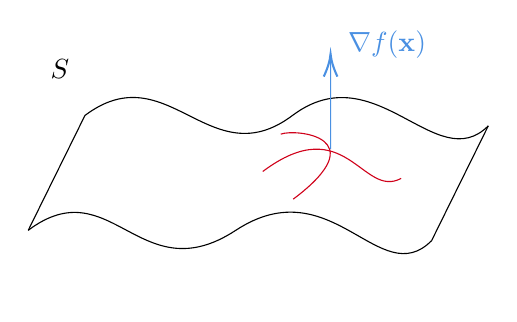
\begin{tikzpicture}[x=0.75pt,y=0.75pt,yscale=-1,xscale=1]
%uncomment if require: \path (0,300); %set diagram left start at 0, and has height of 300

%Curve Lines [id:da603117615542309] 
\draw    (182,133.33) .. controls (222,103.33) and (242,163.33) .. (282,133.33) .. controls (322,103.33) and (351.33,163.33) .. (376.33,138.33) ;
%Curve Lines [id:da030806806310122115] 
\draw    (154.67,188.67) .. controls (194.67,158.67) and (208.33,219) .. (254.67,188.67) .. controls (301,158.33) and (324,218.67) .. (349,193.67) ;
%Straight Lines [id:da891425558098866] 
\draw    (182,133.33) -- (154.67,188.67) ;
%Straight Lines [id:da3777746705205005] 
\draw    (376.33,138.33) -- (349,193.67) ;
%Curve Lines [id:da966844915291705] 
\draw [color={rgb, 255:red, 208; green, 2; blue, 27 }  ,draw opacity=1 ]   (267.67,160.33) .. controls (307.67,130.33) and (315.67,173.67) .. (334.33,163.67) ;
%Straight Lines [id:da4872470345315718] 
\draw [color={rgb, 255:red, 74; green, 144; blue, 226 }  ,draw opacity=1 ]   (300.38,149.51) -- (300.34,105.67) ;
\draw [shift={(300.33,103.67)}, rotate = 449.94] [color={rgb, 255:red, 74; green, 144; blue, 226 }  ,draw opacity=1 ][line width=0.75]    (10.93,-3.29) .. controls (6.95,-1.4) and (3.31,-0.3) .. (0,0) .. controls (3.31,0.3) and (6.95,1.4) .. (10.93,3.29)   ;
%Curve Lines [id:da2744551672083855] 
\draw [color={rgb, 255:red, 208; green, 2; blue, 27 }  ,draw opacity=1 ]   (282.33,173.67) .. controls (322.33,143.67) and (283.67,139.67) .. (276.33,142.33) ;

% Text Node
\draw (164.21,105.31) node [anchor=north west][inner sep=0.75pt]    {$S$};
% Text Node
\draw (307.54,91.31) node [anchor=north west][inner sep=0.75pt]  [color={rgb, 255:red, 74; green, 144; blue, 226 }  ,opacity=1 ]  {$\nabla f(\mathbf{x})$};


\end{tikzpicture}

 \end{center}


 \section{Computing Gradients}

In example in the previous section, computing the gradient was somewhat difficult, requiring various expansions. We might wonder if it possible to compute it more efficiently, in some orthogonal curvilinear coordinates.

In Cartesian coordinates, things are straightforward.
To get the change $\vv{x} \mapsto \vv{x} + \vv{h}$, we could just get the change $x \mapsto x + h_1$, $y \mapsto y + h_2$, $z \mapsto z + h_3$, then
\begin{align*}
f(\vv{x} + \vv{h}) &= f(x + h_1, y + h_2, z + h_3) \\
				   &= f(\vv{x}) + \frac{\partial f}{\partial x} h_1 + \frac{\partial f}{\partial y} h_2  + \frac{\partial f}{\partial z} h_3 + o(\vv{h}) \\
				   &= f(\vv{x}) +  \begin{pmatrix}
					\partial f / \partial x \\
					\partial f / \partial y \\
					\partial f / \partial z 
				   \end{pmatrix} \cdot \vv{h} + o(\vv{h}),
\end{align*}
so
$$
\nabla f = \begin{pmatrix}
	\partial f / \partial x \\
	\partial f / \partial y \\
	\partial f / \partial z 
   \end{pmatrix}.
$$
Or, using suffix notation, 
$$
\nabla f = \vv{e}_i \frac{\partial f}{\partial x_i}, \quad \text{or} \quad [\nabla f]_i = \frac{\partial f}{\partial x_i}.
$$
We can see that $\nabla$ is a kind of vector differential operator.

So let's try and see how to apply this to other coordinate systems. Recall that in Cartesian coordinates, the line element was
$$
\dd \vv x = \dd x \vv{e}_x + \dd y \vv{e}_y + \dd z \vv{e}_z = \dd x_i \vv{e}_i.
$$
Also a function $f = f(x, y, z)$ has differential
$$
\dd f = \frac{\partial f}{\partial x_i} \dd x_i.
$$
Then
\begin{align*}
	\nabla f \cdot \dd{x} &= \left(\vv{e}_i \frac{\partial f}{\partial x_i}\right) \cdot (\vv{e}_j \dd x_j) \\
	&= \frac{\partial f}{\partial x_i} \underbrace{\vv{e}_i \cdot \vv{e}_j}_{\delta_{ij}} \; \dd x_j \\
	&= \frac{\partial f}{\partial x_i} \; \dd x \\
	&= \dd f.
\end{align*}
So we have the following important result:
$$
\boxed{\nabla f \cdot \dd x = \dd f}
$$
This result is important because it is \emph{coordinate independent}.

\begin{remark}[Abuse of Notation]
	So far we have jumped from writing $f(\vv{x}) \rightarrow f(x, y, z)$. Really, what we should have written is $F(x, y, z) = f(\vv{x, y, z})$. This seems over the top in Cartesian coordinates, but would be far more proper to write $F(u, v, w) = f(\vv{x}(u, v, w))$.
\end{remark}

\begin{proposition}
	If $(u, v, w)$ are orthogonal curvilinear coordinates, and $f = f(u, v, w)$. Then
	$$
	\nabla f = \frac{1}{h_u} \frac{\partial f}{\partial u} \vv{e}_u + \frac{1}{h_v} \frac{\partial f}{\partial v} \vv{e}_v + \frac{1}{h_w} \frac{\partial f}{\partial w} \vv{e}_w.
	$$
\end{proposition}
\begin{proof}
	If $f = f(u, v, w)$ and $\vv{x} = \vv{x}(u, v, w)$, then
	$$
\dd f = \frac{\partial f}{\partial u} \dd u + \frac{\partial f}{\partial v} \dd v + \frac{\partial f}{\partial w} \dd w,
	$$
	and
	$$
	\dd \vv{x} = h_u \dd u \vv{e}_u + h_v \dd v \vv{e}_v + h_w \dd w \vv{e}_w.
	$$
	Using $\dd f = \nabla \cdot \dd \vv{x}$,  and writing
	$$
	\nabla f = [\nabla f]_u \vv{e}_u + [\nabla f]_v \vv{e}_v + [\nabla f]_w \vv{e}_w,
	$$
	we find that
	$$
	\frac{\partial f}{\partial u} \dd u + \frac{\partial f}{\partial v} \dd v + \frac{\partial f}{\partial w} \dd w = h_u [\nabla f]_u \dd u + h_v [\nabla f]_v \dd v + h_w [\nabla f]_w \dd w.
	$$
	Since $\{\dd u, \dd v, \dd w\}$ are linearly independent, we can compare components, and we get 
	$$
	[\nabla f]_u = \frac{1}{h_u} \frac{\partial f}{\partial u},
	 \quad [\nabla f]_v = \frac{1}{h_v} \frac{\partial f}{\partial v}, 
	\quad [\nabla f]_w = \frac{1}{h_w} \frac{\partial f}{\partial w},
	$$
	as required.
\end{proof}

\begin{example}[Gradient in Cyclindrical/Spherical Coordinates]
	In cylindrical polar coordinates $(\rho, \phi, z)$, we have $h_\rho = 1$, $h_\phi = \rho$, and $h_z = 1$. So
	$$
	\nabla f = \frac{\partial f}{\partial \rho} \vv{e}_\rho + \frac{1}{\rho}\frac{\partial f}{\partial \phi} \vv{e}_\phi + \frac{\partial f}{\partial z} \vv{e}_z.
	$$

	In spherical polar coordinates $(r, \theta, \phi)$, we have $h_r = 1$, $h_\theta = r$ and $h_\phi = r \sin \theta$. Then
	$$
\nabla f = \frac{\partial f}{\partial r} \vv{e}_r + \frac{1}{r} \frac{\partial f}{\partial \theta} \vv{e}_\theta + \frac{1}{ r \sin \theta} \frac{\partial f}{\partial \phi} \vv{e}_\phi.
	$$
\end{example}

\chapter{Integration over Lines, Surfaces and Volumes}

We are now going to move on to the other (possibly more interesting) side of Calculus -- integration! We are going to study how integration can be performed over various objects, beginning with lines (a rather simple generalization of `normal' integration), followed by surfaces and volumes.

\section{Line Integrals}

We will begin by defining the line integral.

\begin{definition}[Line Integral]
	For a vector field $\vv{F} = \vv{F}(\vv{x})$ and a piecewise smooth parameterized curve $t \mapsto \vv{x}(t)$ with $t \in [a, b]$, we define the \vocab{line integral}
	$$
	\int_C \vv{F} \cdot \dd \vv{x} = \int_a^b \vv{F}(\vv{x}(t)) \cdot \frac{\dd \vv{x}}{\dd t} \dd t
 	$$
\end{definition}

Note that the direction is important (we integrate over `increasing $t$'). If we wanted to integrate in the opposite direction over the curve, we would consider $\int_{-C}$.

\begin{example}
	\label{ex:q}
	Consider the vector field 
	$$
	\vv{F} = \begin{pmatrix}
		x^2 y \\ yz \\ 2zx
	\end{pmatrix},
	$$
	and consider two curves connecting the origin to $(1, 1, 1)$,
	\begin{align*}
		C_1: t \longmapsto \begin{pmatrix}
			t \\ t\\ t
		\end{pmatrix}, \quad t \in [0, 1], \quad \quad
		C_2: t \longmapsto \begin{pmatrix}
			t \\ t\\ t^2
		\end{pmatrix}, \quad t \in [0, 1].
	\end{align*}
	So
	$$
	\int_{C_1} \vv{F} \cdot \dd \vv{x}= \int_0^1 \begin{pmatrix}
		t^3 \\ t^2\\ 2t^2
	\end{pmatrix} \cdot \begin{pmatrix}
		1 \\ 1\\ 1
	\end{pmatrix} \dd t = \frac{5}{4}.
	$$
	and
	$$
	\int_{C_2} \vv{F} \cdot \dd \vv{x}= \int_0^1 \begin{pmatrix}
		t^3 \\ t^2\\ 2t^2
	\end{pmatrix} \cdot \begin{pmatrix}
		1 \\ 1\\ 2t
	\end{pmatrix} \dd t = \frac{13}{10}.
	$$
\end{example}

We can see from the above example that the line integral between two points depends on the path taken.

\begin{example}
	A particle at $\vv{x}$ experiences a force in cylindrical polars of
	$$
	\vv{F}(\vv{x}) = x \rho \vv{e}_{\phi}.
	$$
	We will calculate the work done by travelling along
	$$
	C: t \longmapsto \begin{pmatrix}
		a \cos t \\ a \sin t \\ t
	\end{pmatrix}, \quad t \in [0, 2\pi].
	$$

	Recall the line element in cylindrical polars is
	$$
	\dd \vv{x} = \dd \rho \vv{e}_{\rho} + \rho \dd \phi \vv{e}_{\phi} + \dd z \vv{e}_z.
	$$
	So
	$$
\vv{F} \cdot \dd x = z \rho^2 \dd \phi.
	$$
	Also on the path $(\rho, \phi, z) = (a, t, t)$, so $(\dd \rho, \dd \phi, \dd z) = (0, \dd t, \dd t)$. So $\vv{F} \cdot \dd \vv{x} = a^2 t \dd t$. Finally,
	$$
	\int_C \vv{F} \cdot \dd \vv{x} = a^2 \int_0^{2 \pi} t \dd t = 2 \pi^2 a^2
	$$
\end{example}

A curve $\vv{x}(t)$ with $t \in [a, b]$ might be such that $\vv{x}(a) \vv{x}(b)$, that is, the curve is \emph{closed}. In this case, we write
$$
\oint_C \vv{F} \cdot \dd \vv{x}.
$$
Sometimes we call integrals of this form the $\vocab{circulation}$ of $\vv{F}$ about $C$.

\begin{example}
	Using $C_1$ and $C_2$ from \autoref{ex:q}, we define the curve $C = C_1 - C_2$. Then
	$$
		\oint_C \vv{F} \cdot \dd \vv{x} = \int_{C_1} \vv{F} \cdot \dd \vv{x} - \int_{C_2} \vv{F} \cdot \dd \vv{x} = - \frac{2}{15}.
	$$
\end{example}

\section{Conservative Forces and Exact Differentials}

We have seen how to interpret things like $\vv{F} \cdot \dd \vv{x}$ when they're inside an integral. This is another differential form, that is, in coordinates $(u, v, w)$,
$$
\vv{F} \cdot \dd x = (\ )\dd u + (\ ) \dd v + (\ ) \dd w,
$$
where there's \emph{something} inside the brackets.

\begin{definition}[Exactness]
	We say that $\vv{F} \cdot\dd \vv{x}$ is \vocab{exact} if
	$
	\vv{F} \cdot \dd \vv{x} = \dd f,
	$
	for some scalar function $f$.
\end{definition}

Recall that $\dd f = \nabla f \cdot \dd \vv{x}$, so $\vv{F} \cdot \dd \vv{x}$ is exact if and only if $\vv{F} = \nabla f$ for some scalar function $f$. We call such vector fields \vocab{conservative}.


For a vector field $\vv{F}$, we have $\vv{F} \cdot \dd \vv{x}$ is exact if and only if $\vv{F}$ is conservative.

Using properties such as $\dd(\alpha f + \beta g) = \alpha \dd f + \beta \dd g$ for constant $\alpha, \beta$ and $\dd(fg) = g \dd f + f \dd g$, usually it is easy to see if a differential form $\vv{F} \cdot \dd \vv{x}$ is exact.

\begin{proposition}
	If $\theta$ is an exact differential form, then
	$$
	\oint_C \theta = 0,
	$$
	for any closed curve $C$.
\end{proposition}
\begin{proof}
	If $\theta$ is exact, then $\theta = \nabla f \cdot \dd \vv{x}$ for some scalar $f$. If $C: t \mapsto \vv{x}(t)$ with $t \in [a, b]$,
	\begin{align*}
		\oint_C \theta &= \oint_C \nabla f \cdot \dd \vv{x} \\
			&= \int_{a}^b \nabla f(\vv{x}(t)) \cdot \frac{\dd \vv{x}}{\dd t} \dd t \\
			&= \int_a^b \frac{\dd}{\dd t} \left[f(\vv{x}(t))\right] \dd t \\
			&= f(\vv{x}(a)) - f(\vv{x}(b))\\
			&= 0,
	\end{align*}
	if $\vv{x}(a) = \vv{x}(b)$.
\end{proof}

Equivalently, if $\vv{F}$ is conservative, then the circulation of $\vv{F}$ around any closed loop curve $C$ vanishes,  $\oint_C \vv{F} \cdot \dd \vv{x} = 0$.

Also if $\vv{F}$ is conservative (and $\vv{F} \cdot \dd \vv{x}$ is exact), then the line integral between points $A = \vv{x}(a)$ and $B = \vv{x}(b)$ is \emph{independent} of path.

Now let $(u, v, w)$ be an arbitrary set of orthonormal curvilinear coordinates. Let
$$
\vv{F} \cdot \dd \vv x = \theta = \underbrace{A(u, v, w)}_{\theta_1} \dd u + \underbrace{B(u, v, w)}_{\theta_2} \dd v + \underbrace{C(u, v, w)}_{\theta_3} \dd w = \theta_i \dd u_i.
$$
A \emph{necessary} condition for $\theta$ to be exact is
$$
	\frac{\partial \theta_i}{\partial u_j} = \frac{\partial \theta_j}{\partial u_i}, \quad \quad \text{for each }i, j.
$$
Indeed, if $\theta$ is exact, then $\theta = \dd f$ for some $f$. Then
\begin{equation}\label{eq:closed}
	\theta = \frac{\partial f}{\partial u_i} \dd u_i \iff \theta_i = \frac{\partial f}{\partial u_i},\tag{$*$}
\end{equation}
and so
$$
	\frac{\partial \theta_i}{\partial u_j} = \frac{\partial^2 f}{\partial u_j \partial u_i} = \frac{\partial^2 f}{\partial u_i \partial u_j} = \frac{\partial \theta_j}{ \partial u_i}.
$$

If a differential form satisfies \eqref{eq:closed}, we call it \vocab{closed}. So if $\theta$ is exact, then $\theta$ is closed.

The reverse implication is true if the domain $\Omega \subset \R^3$ on which $\theta$ is defined is simply-connected\footnote{All closed loops in $\Omega$ can be `continuously shrunk' to any point inside $\Omega$ without leaving it.}

\begin{example}
	Consider $\theta = y \dd x - x \dd y$. We will check if it is closed. If so, we need to have
	$$
	\frac{\partial y}{\partial y} = \frac{\partial -x}{\partial x},
	$$
	which is clearly not the case, as $1 \neq -1$. Thus $\theta$ is not exact.
\end{example}

\begin{example}[Silly Example]
	We will compute the line integral
	$$
	\oint_C 3x^2 y \dd x + x^3 \dd y,
	$$
	over the curve
	$$
	C: t \mapsto \begin{pmatrix}
		\cos(\im(\zeta(1/2 + it))) \\
		\sin(\re(\zeta(1/2 + it))) \\
		0
	\end{pmatrix}, \quad \quad t \in [\alpha_1, \alpha_{100}],
	$$
	where $\alpha_1$ and $\alpha_{100}$ are the 1st and 100th zero of $\zeta(1/2 + it)$, so that $\zeta(1/2 + i \alpha_1) = \zeta(1.2 + i \alpha_{100}) = 0$.
	
	Now this differential form $d(x^3 y)$, and this is a closed curve, thus $\oint_C 3x^2 y \dd x + x^3 \dd y = 0$.
\end{example}

\section{Integration in $\R^2$}

We want to integrate over some bounded region say $D \subset \R^2$. To do this, we will cover $D$ with small, disjoint sets $A_{ij}$, each with area $\delta A_{ij}$, so that each of these are contained in a disk of radius $\epsilon > 0$.
Let $(x_i, y_j)$ be points contained in each $A_{ij}$.

Now define
$$
	\int_D f(\vv{x}) \dd A = \lim_{\epsilon \to 0} \sum_{i,j} f(x_i, y_j) \delta A_{ij}
$$
We will say that the integral exists if it is independent of our choice of $A_{ij}$ and choice of $(x_i, y_j)$.

An obvious choice of partition would be to use rectangles with $\delta A_{ij} = \delta x \delta y$. We could sum over horizontal strips of width $\delta y$, then take the limit as $\delta x \rightarrow 0$. This gives
$$
	\delta y \int_{x_y} f(x, y) \dd x,
$$
where $X_y = \{x \mid (x, y) \in D \}$. Summing over each such strip, we'd end up with
$$
\int_{D} f(x, y) \dd A = \int_Y \left(\int_{X_y} f(x, y) \dd x\right) \dd u,
$$
where $Y$ is as in the diagram below.

\begin{center}
	

\tikzset{every picture/.style={line width=0.75pt}} %set default line width to 0.75pt        

\begin{tikzpicture}[x=0.75pt,y=0.75pt,yscale=-1,xscale=1]
%uncomment if require: \path (0,300); %set diagram left start at 0, and has height of 300

%Straight Lines [id:da1629034885697126] 
\draw    (200,210) -- (418,210) ;
\draw [shift={(420,210)}, rotate = 180] [color={rgb, 255:red, 0; green, 0; blue, 0 }  ][line width=0.75]    (10.93,-3.29) .. controls (6.95,-1.4) and (3.31,-0.3) .. (0,0) .. controls (3.31,0.3) and (6.95,1.4) .. (10.93,3.29)   ;
%Straight Lines [id:da31151739933589306] 
\draw    (210,220) -- (210,22) ;
\draw [shift={(210,20)}, rotate = 450] [color={rgb, 255:red, 0; green, 0; blue, 0 }  ][line width=0.75]    (10.93,-3.29) .. controls (6.95,-1.4) and (3.31,-0.3) .. (0,0) .. controls (3.31,0.3) and (6.95,1.4) .. (10.93,3.29)   ;
%Shape: Polygon Curved [id:ds10249847549557578] 
\draw   (250,90) .. controls (270,80) and (360,70) .. (340,90) .. controls (320,110) and (320,120) .. (340,150) .. controls (360,180) and (270,180) .. (250,150) .. controls (230,120) and (230,100) .. (250,90) -- cycle ;
%Straight Lines [id:da25451399177896894] 
\draw  [dash pattern={on 0.84pt off 2.51pt}]  (321,78) -- (210,78) ;
%Straight Lines [id:da041739869365173266] 
\draw  [dash pattern={on 0.84pt off 2.51pt}]  (309,173) -- (210,173) ;
%Shape: Brace [id:dp6621245674606429] 
\draw   (210,78.75) .. controls (205.33,78.72) and (202.99,81.04) .. (202.96,85.71) -- (202.81,115.71) .. controls (202.77,122.38) and (200.42,125.7) .. (195.75,125.68) .. controls (200.42,125.7) and (202.73,129.04) .. (202.7,135.71)(202.72,132.71) -- (202.54,165.71) .. controls (202.52,170.38) and (204.84,172.72) .. (209.51,172.75) ;
%Straight Lines [id:da07321232057182314] 
\draw [color={rgb, 255:red, 208; green, 2; blue, 27 }  ,draw opacity=1 ]   (239,130) -- (328,130) ;
%Straight Lines [id:da3528968860450654] 
\draw [color={rgb, 255:red, 208; green, 2; blue, 27 }  ,draw opacity=1 ]   (237,124) -- (326,124) ;
%Straight Lines [id:da29786796871231136] 
\draw    (380,130) -- (331,127.12) ;
\draw [shift={(329,127)}, rotate = 363.37] [color={rgb, 255:red, 0; green, 0; blue, 0 }  ][line width=0.75]    (10.93,-3.29) .. controls (6.95,-1.4) and (3.31,-0.3) .. (0,0) .. controls (3.31,0.3) and (6.95,1.4) .. (10.93,3.29)   ;
%Straight Lines [id:da30084043292662677] 
\draw  [dash pattern={on 4.5pt off 4.5pt}]  (239,130) -- (239,210) ;
%Straight Lines [id:da7980958464242905] 
\draw  [dash pattern={on 4.5pt off 4.5pt}]  (328,130) -- (328,210) ;
%Shape: Brace [id:dp5081444039097228] 
\draw   (239,210.75) .. controls (239.03,215.42) and (241.37,217.74) .. (246.04,217.71) -- (273.29,217.56) .. controls (279.96,217.52) and (283.3,219.83) .. (283.33,224.5) .. controls (283.3,219.83) and (286.62,217.48) .. (293.29,217.45)(290.29,217.46) -- (320.54,217.29) .. controls (325.21,217.27) and (327.53,214.93) .. (327.5,210.26) ;

% Text Node
\draw (351,63) node [anchor=north west][inner sep=0.75pt]    {$D$};
% Text Node
\draw (181,122) node [anchor=north west][inner sep=0.75pt]    {$Y$};
% Text Node
\draw (382,130) node [anchor=west] [inner sep=0.75pt]    {$\delta y$};
% Text Node
\draw (271,232) node [anchor=north west][inner sep=0.75pt]    {$X_{y}$};


\end{tikzpicture}

\end{center}

If we instead sum over vertical strips, we get 
$$
	\int_D f(x, y) \dd A = \int_X \left(\int_{Y_x} f(x, y) \dd y\right) \dd x.
$$

More concisely, we have
$$
\dd A = \dd x \dd y = \dd y \dd x. 
$$
This is known as Fuibini's theorem (with a few caveats that we won't worry about), which you may see at a much later course.

\begin{example}
	Let $D$ be a triangle with vertices at $(0, 0)$, $(1, 0)$ and $(0, 1)$. 

	\begin{center}
		

\tikzset{every picture/.style={line width=0.75pt}} %set default line width to 0.75pt        

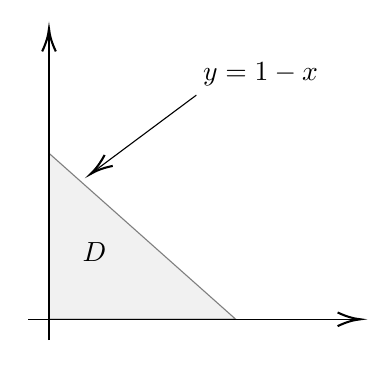
\begin{tikzpicture}[x=0.75pt,y=0.75pt,yscale=-1,xscale=1]
%uncomment if require: \path (0,300); %set diagram left start at 0, and has height of 300

%Shape: Right Triangle [id:dp07296511159724295] 
\draw  [color={rgb, 255:red, 128; green, 128; blue, 128 }  ,draw opacity=1 ][fill={rgb, 255:red, 241; green, 241; blue, 241 }  ,fill opacity=1 ] (210,130) -- (300,210) -- (210,210) -- cycle ;
%Straight Lines [id:da19925281886663593] 
\draw    (200,210) -- (358,210) ;
\draw [shift={(360,210)}, rotate = 180] [color={rgb, 255:red, 0; green, 0; blue, 0 }  ][line width=0.75]    (10.93,-3.29) .. controls (6.95,-1.4) and (3.31,-0.3) .. (0,0) .. controls (3.31,0.3) and (6.95,1.4) .. (10.93,3.29)   ;
%Straight Lines [id:da9848620958169408] 
\draw    (210,220) -- (210,72) ;
\draw [shift={(210,70)}, rotate = 450] [color={rgb, 255:red, 0; green, 0; blue, 0 }  ][line width=0.75]    (10.93,-3.29) .. controls (6.95,-1.4) and (3.31,-0.3) .. (0,0) .. controls (3.31,0.3) and (6.95,1.4) .. (10.93,3.29)   ;
%Straight Lines [id:da6104098831517629] 
\draw    (281,102) -- (231.6,138.81) ;
\draw [shift={(230,140)}, rotate = 323.31] [color={rgb, 255:red, 0; green, 0; blue, 0 }  ][line width=0.75]    (10.93,-3.29) .. controls (6.95,-1.4) and (3.31,-0.3) .. (0,0) .. controls (3.31,0.3) and (6.95,1.4) .. (10.93,3.29)   ;

% Text Node
\draw (225,172) node [anchor=north west][inner sep=0.75pt]    {$D$};
% Text Node
\draw (283,99) node [anchor=south west] [inner sep=0.75pt]    {$y=1-x$};


\end{tikzpicture}

	\end{center}
	If $f(x, y) = xy^2$, then if we integrate over horizontal strips, 
	\begin{align*}
		\int_D f \dd A &= \int_0^1\left(\int_{0}^{1 - y} xy^2 \dd x \right) \dd y\\
	&= \int_0^1 y^2 \left[ \frac{1}{2}x^2 \right]_0^{1 - y} \dd y \\
	&= \int_0^1 \frac{1}{2} y^2 (1 - y)^2 \dd y = \frac{1}{60}.
	\end{align*}
	If we did the same with vertical strips, we could get
	\begin{align*}
		\int_D f \dd A &= \int_0^1 \left(\int_0^{1 - x} xy^2 \dd y\right) \dd x \\
		&= \int_0^1 x \left[\frac{1}{3}y^3\right]_0^{1 - x} \dd x = \frac{1}{60},
	\end{align*}
	and they are the same.
\end{example}

A special case is when $f(x, y) = g(x)h(y)$ and $D$ is a rectangle, $D = \{(x, y) \mid a \leq x \leq b, c \leq y \leq d \}$, then
$$
\int_A f(x, y) \dd A = \left(\int_{a}^b g(x) \dd x\right)\left(\int_c^d h(y) \dd y\right).
$$

It is often useful to introduce a change of variables to compute $\int_a^b f(x) \dd x$.
If we introduce $x = x(u)$ with $x(\alpha) = a$ and $x(\beta) = b$, then
$$
\int_a^b f(x)\dd x = \begin{cases}
	+ \int_\alpha^\beta f(x(u)) \frac{\dd x}{\dd u} \dd u &\mbox{if } \beta > \alpha, \\
	- \int_\beta^\alpha f(x(u)) \frac{\dd x}{\dd u} \dd u  &\mbox{if } \alpha > \beta.
   \end{cases}
$$
So if $I = [a, b]$ and $I = x(I)'$, then
$$
\int_I f(x) \dd x = \int_{I'} f(x(u)) \left|\frac{\dd x}{\dd u}\right| \dd u.
$$

There is a similar formula in two dimensions.

\begin{proposition}
	Let $x = x(u, v)$ and $y = y(u, v)$ be a smooth, invertible transformation with smooth inverse that maps the region $D'$ in the $(u, v)$ plane to the region $D$ in the $(x, y)$-plane.
	Then
	$$
	\int_D f(x, y) \dd x \dd y = \int_{D'} f(x(u, v), y(u, v)) \left|\frac{\partial(x, y)}{\partial(u, v)}\right| \dd u \dd v,
	$$
	where
	$$
	\frac{\partial (x, y)}{\partial (u, v)} = \det\begin{pmatrix}
		\partial x/\partial u & \partial x / \partial v \\
		\partial y / \partial u & \partial y / \partial v
	\end{pmatrix}
	$$
	is the \emph{Jacobian}, often denoted by $J$.
\end{proposition}

The short version is that $\dd x \dd y = |J| \dd u \dd v$.

\begin{example}
	Using polar coordinates $(\rho, \phi)$,
	$$
	x(\rho, \phi) = \rho \cos \phi, \quad \quad y(\rho, \phi) = \rho \sin \phi.
	$$
	Hence 
	$$
	J = \det \begin{pmatrix}
		\cos \phi & - \rho \sin \phi \\
		\sin \phi & \rho \cos \phi
	\end{pmatrix} = \rho,
	$$
	So if $D = \{(x, y)  \mid x > 0, y > 0, x^2 + y^2 < R^2 \}$, then $D' = \{(\rho, \phi) \mid 0 < \rho < R, 0 < \phi < \pi/2\}$, and
	$$
	\int_D f(x, y) \dd x\ \dd y = \int_{D'} f(\rho \cos \phi, \rho \sin \phi) \rho\  \dd \rho \dd \phi,
	$$
	so $\dd x \dd y = \rho \dd \rho \dd \phi$.

	Taking $R \rightarrow \infty$, we get
	$$
	\int_{x = 0}^{\infty} \int_{y = 0}^{\infty} f(x, y) \dd y = \int_{\phi = 0}^{\pi/2} \int_{\rho = 0}^{\infty} f(\rho \cos \phi, \rho \sin \phi) \rho \; \dd \rho \dd\phi.
	$$

	Now consider $I = \int_0^{\infty} e^{-x^2} \dd x$. Using the previous result, we have
	\begin{align*}
		I^2 &= \int_{0}^{\infty} e^{-x^{2}} \dd x \cdot \int_{0}^{\infty} e^{-y^{2}} \dd y \\
			&= \int_{x=0}^{\infty} \int_{y=0}^{\infty} e^{-x^{2}-y^{2}} \dd x \dd y \\
			&= \int_{\phi = 0}^{\pi/2} \left(\int_{\rho}^{\infty} e^{- \rho^2} \rho \dd\rho \right) \dd \phi \\
			&= \frac{\pi}{2} \int_0^{\infty} \frac{\dd}{\dd \rho} \left(-\frac{1}{2} e^{- \rho^2}\right) \dd \rho = \frac{\pi}{4}.
	\end{align*}
	Thus $I = \frac{\sqrt{\pi}}{2}$.
\end{example}

\section{Integration in $\R^3$}

To integrate over a region $V$ in $\R^3$, we use similar ideas to that of the previous section. Let
$$
	\int_V f(\vv{x}) \dd V = \lim_{\epsilon \to 0} \sum_{i, j, k} f(x_i, y_j, z_k) \delta V_{ijk},
$$
where the \emph{volume element} satisfies
$$
\dd V = \dd x \ \dd y \ \dd z.
$$
We can do the integrals in any order (again Fuibini's theorem).

\begin{example}
	Consider the region $V$ bound by planes $x + y + z = 1$ and $x = 0, y = 0$ and $z = 0$. We will find the volume (integrating $1$ over the region).
	\begin{center}
		

\tikzset{every picture/.style={line width=0.75pt}} %set default line width to 0.75pt        

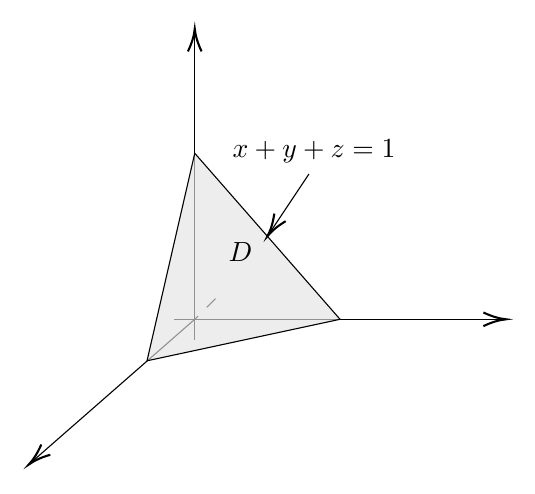
\begin{tikzpicture}[x=0.75pt,y=0.75pt,yscale=-1,xscale=1]
%uncomment if require: \path (0,300); %set diagram left start at 0, and has height of 300

%Straight Lines [id:da7142734641721928] 
\draw    (200,210) -- (358,210) ;
\draw [shift={(360,210)}, rotate = 180] [color={rgb, 255:red, 0; green, 0; blue, 0 }  ][line width=0.75]    (10.93,-3.29) .. controls (6.95,-1.4) and (3.31,-0.3) .. (0,0) .. controls (3.31,0.3) and (6.95,1.4) .. (10.93,3.29)   ;
%Straight Lines [id:da7321899041114295] 
\draw    (210,220) -- (210,72) ;
\draw [shift={(210,70)}, rotate = 450] [color={rgb, 255:red, 0; green, 0; blue, 0 }  ][line width=0.75]    (10.93,-3.29) .. controls (6.95,-1.4) and (3.31,-0.3) .. (0,0) .. controls (3.31,0.3) and (6.95,1.4) .. (10.93,3.29)   ;
%Straight Lines [id:da3568532467086144] 
\draw    (210,210) -- (131.51,278.68) ;
\draw [shift={(130,280)}, rotate = 318.81] [color={rgb, 255:red, 0; green, 0; blue, 0 }  ][line width=0.75]    (10.93,-3.29) .. controls (6.95,-1.4) and (3.31,-0.3) .. (0,0) .. controls (3.31,0.3) and (6.95,1.4) .. (10.93,3.29)   ;
%Straight Lines [id:da2728884008736586] 
\draw  [dash pattern={on 4.5pt off 4.5pt}]  (220,200) -- (210,210) ;
%Shape: Polygon [id:ds4065449031533396] 
\draw  [fill={rgb, 255:red, 227; green, 227; blue, 227 }  ,fill opacity=0.64 ] (280,210) -- (187,230) -- (210,130) -- cycle ;
%Straight Lines [id:da8133123312139356] 
\draw    (265,140) -- (246.11,168.34) ;
\draw [shift={(245,170)}, rotate = 303.69] [color={rgb, 255:red, 0; green, 0; blue, 0 }  ][line width=0.75]    (10.93,-3.29) .. controls (6.95,-1.4) and (3.31,-0.3) .. (0,0) .. controls (3.31,0.3) and (6.95,1.4) .. (10.93,3.29)   ;

% Text Node
\draw (225,172) node [anchor=north west][inner sep=0.75pt]    {$D$};
% Text Node
\draw (227,122) node [anchor=north west][inner sep=0.75pt]    {$x+y+z=1$};


\end{tikzpicture}

	\end{center} 
We have
\begin{align*}
	\int_V \dd V &= \int_{x = 0}^1 \left(\int_{y = 0}^{1 - x} \left(\int_{z = 0}^{1 - x - y} \dd z\right) \dd y\right) \dd x \\
	&= \int_{x = 0}^{1} \int_{y = 0}^{1 - x}(1 - x - y) \dd y  \\
	&= \frac{1}{6}.
\end{align*}

If we wanted to compute say the center of mass, then assuming it had constant density say $\rho = 1$, the center of mass $X$ is
$$
X = \frac{1}{M} \int_V \rho \vv{x} \dd V = \frac{1}{4}\begin{pmatrix}
	1\\ 1\\ 1
\end{pmatrix}
$$
\end{example}

We can write down the change of variables for three dimensional integrals.

\begin{proposition}
	Let $x = x(u, v, w)$, $y = y(u, v, w)$ and $z = z(u, v, w)$ be a continuously differentiable bijection with continuously differentiable inverse tht mps the volume $V'$ to $V$. Then
	$$
	\int_V f(x, y, z) \dd x \ \dd y \ \dd z = \int_{V'} f(x(u, v, w), y(u, v, w), z(u, v, w)) |J| \dd u\  \dd v\ \dd w,
	$$
	where
	$$
	J = \frac{\partial(x, y, z)}{\partial(u, v, w)}
	$$
\end{proposition}
Again the short version is $\dd x\ \dd y\ \dd z = |J| \dd u\ \dd v\ \dd w$.

\begin{example}
	In cylindrical polars $(u, v, w) = (\rho, \phi, z)$,
	$$
	\dd V = \rho \; \dd\rho \; \dd \phi \; \dd z,
	$$
	and $|J| = \rho$.

	In spherical polars $(u, v, w) = (r, \theta, \phi)$,
	$$
	\dd V = r^2 \sin \theta \; \dd r \; \dd \theta \; \dd \phi,
	$$
	and $|J| = r^2 \sin \theta$.
\end{example}

\begin{example}
	Suppose we wanted to calculate the volume of the ball of radius $R$, $V = \{(x, y, z) \mid x^2 + y^2 + z^2 \leq R^2\}$. 
	
	We could try a `bare hands' approach in Cartesian coordinates.
	\begin{align*}
		&\ \int_V \dd V\\ &= \int_{z=-R}^{R} \left(\int_{y = - \sqrt{R^2 - z^2}}^{\sqrt{R^2 - z^2}} \left( \int_{x = - \sqrt{R^2 - z^2 - y^2}}^{\sqrt{R^2 - z^2 - y^2}} \dd x\right)\dd y\right)\dd z \\
		&=\int_{z=-R}^{R}\left[\int_{y=-\sqrt{R^{2}-z^{2}}}^{\sqrt{R^{2}-z^{2}}} 2 \sqrt{R^{2}-z^{2}-y^{2}}\; \dd y\right] \;\dd z\\
		&= \int_{z = -R}^{R}\left[y \sqrt{R^2 - z^2 - y^2} + (R^2 - z^2)\tan^{-1}\left(\frac{y}{\sqrt{R^2 - z^2 - y^2}}\right)\right]_{-\sqrt{R^2 - z^2}}^{\sqrt{R^2 - z^2}} \dd z \\
		&= \int_{-R}^R \pi (R^2 - z^2) \dd z = \frac{4 \pi R^3}{3}.
	\end{align*}

	Alternatively, since we have even a limited amount of self respect, we can use spherical polars. We have $V' = \{(r, \theta, \phi) \mid 0 \leq r \leq R, 0 \leq \theta \leq \pi, 0 \leq \phi < 2\pi\}$. Then
	\begin{align*}
		\int_V \dd V &= \int_{\phi=0}^{2 \pi}\left[\int_{\theta=0}^{\pi}\left[\int_{r=0}^{R} r^{2} \sin \theta \; \dd r\right] \dd \theta\right] \dd \phi \\
		&= \int_{\theta=0}^{\pi} \frac{2 \pi R^{3}}{3} \sin \theta \dd\theta = \frac{4 \pi R^3}{3}.
	\end{align*}
	And this is clearly much nicer.
\end{example}

\begin{example}
	Consider a ball of radius $a$ with a cylinder of radius $b < a$ removed. The symmetry suggests that we use cylindrical polar coordinates. In Cartesian coordinates, we would have
	$$
	V = \{(x, y, z) \mid x^2 + y^2 + z^2 \leq a^2, x^2 + y^2 \geq b^2 \},
	$$
	but in cylindrical polars we would have
	$$
	V' = \{(\rho, \phi, z) \mid b \leq \rho \leq a, 0 \leq z^2 + \rho^2 \leq a^2, 0 \leq \phi < 2 \pi\}.
	$$
	So we have
	\begin{align*}
		\int_V \dd V &= \int_{\rho=b}^a \left[\int_{\phi = 0}^{2\pi}\left[\int_{z = -\sqrt{a^2 - \rho^2}}^{\sqrt{a^2 - \rho^2}}\dd t\right]\dd \phi\right]\rho \dd \rho \\
		&= 2 \pi \int_{b}^a 2\rho\sqrt{a^2 - \rho^2} \dd \rho \\
		&= \frac{4 \pi}{3}(a^2 - b^2)^{3/2}.
	\end{align*}
\end{example}

\section{Integration Over Surfaces}

A two dimensional surface in $\R^3$ can be defined implicitly using a function $f : \R^3 \rightarrow \R$.


\end{document} 
